\documentclass[12pt]{article}
%--------------------   start of the 'preamble'
%
\usepackage{graphicx,amssymb,amstext,amsmath,color}
\usepackage[margin=2cm]{geometry}
\usepackage{abstract}
\usepackage{setspace}
\usepackage[footnotesize,bf]{caption}

% TABLE
\usepackage{multicol,hhline,colortbl,multirow}
\usepackage{braket}
\usepackage{siunitx}
\usepackage{hyperref}
\usepackage{authblk}
\usepackage{siunitx}
\usepackage{mathrsfs}
%%\usepackage[sort&compress]{natbib}
%%\bibpunct{(}{)}{,}{a}{, }{;}
%
\usepackage[sort&compress]{natbib}
\bibpunct{[}{]}{,}{s}{}{;}


\definecolor{gray}{gray}{0.8}
\def\mobunits{\square\centi\meter\per\volt\per\second}
\def\gcm{\gram\per\cubic\centi\meter}
\def\ccg{\cellcolor{gray}}

\renewcommand{\labelitemii}{$\circ$}
\renewcommand{\bibname}{References}


\title{MorphCT Results - PAHs}
\author{Matthew Jones}
\date{\today}

\begin{document}
\maketitle


\section{Latest Jobs, 11/17}


Based on the recent changes to the neighbour calculations and fine-graining, I have rerun our PAH stack systems to see if there are any changes.


\section{Mobility Results}


\begin{center}
\begin{tabular}{| c | c | c | c | c | c | c |}
\hline
\rule{0pt}{2.5ex} 
\multirow{2}{*}{\textbf{ID}}&\multirow{2}{*}{\textbf{Simulation Name}}&\textbf{Density}&\textbf{Anisotropy}&\textbf{Anisotropy}&\textbf{Stacks}&\textbf{Mobility}\\
                            &&(\SI{}{\gcm})&(Arb. U.)&(Shape)&(Arb. U.)&(\SI{}{\mobunits})\\
\hhline{|=======|}
\textbf{\ccg1}&\rule{0pt}{2.5ex}\ccg PE\_MultiStack\_Eclipsed&\ccg 1.06&\ccg 0.9456&\ccg Thin Tube&\ccg19&\ccg5.87$\times 10^{0}$\\
\textbf{2}&\rule{0pt}{2.5ex}PE\_SingleStack\_Eclipsed&1.06&0.0206&Spherical&8&$1.13\times 10^{-1}$\\
\textbf{\ccg3}&\rule{0pt}{2.5ex}\ccg PE\_SingleStack\_Ordered&\ccg 1.06&\ccg 0.1087&\ccg Oblate Spheroid&\ccg16&\ccg5.44$\times 10^{-1}$\\
\hhline{|=======|}
\textbf{4}&\rule{0pt}{2.5ex}PT\_MultiStack\_Eclipsed&1.01&0.0581&Spherical&20&8.80$\times 10^{-1}$\\
\textbf{\ccg5}&\rule{0pt}{2.5ex}\ccg PT\_MultiStack\_Ordered&\ccg 1.01&\ccg 0.1414&\ccg Oblate Spheroid&\ccg20&\ccg2.49$\times 10^{-2}$\\
\textbf{6}&\rule{0pt}{2.5ex}PT\_SingleStack\_Eclipsed&1.01&0.7264&Thin Tube&1&1.15$\times 10^{0}$\\
\textbf{\ccg7}&\rule{0pt}{2.5ex}\ccg PT\_SingleStack\_Ordered&\ccg 1.01&\ccg 0.0575&\ccg Sphere&\ccg1&\ccg4.91$\times 10^{0}$\\
\hhline{-------}
\end{tabular}\label{table:mob}
\captionof{table}{The results from MorphCT for the various PAH morphologies. See the below section for a discussion of the stacks.}
\end{center}

\clearpage


The mobility results are effectively the same, although some of the anisotropy values have changed from previously.


\begin{figure}[h]\centering
	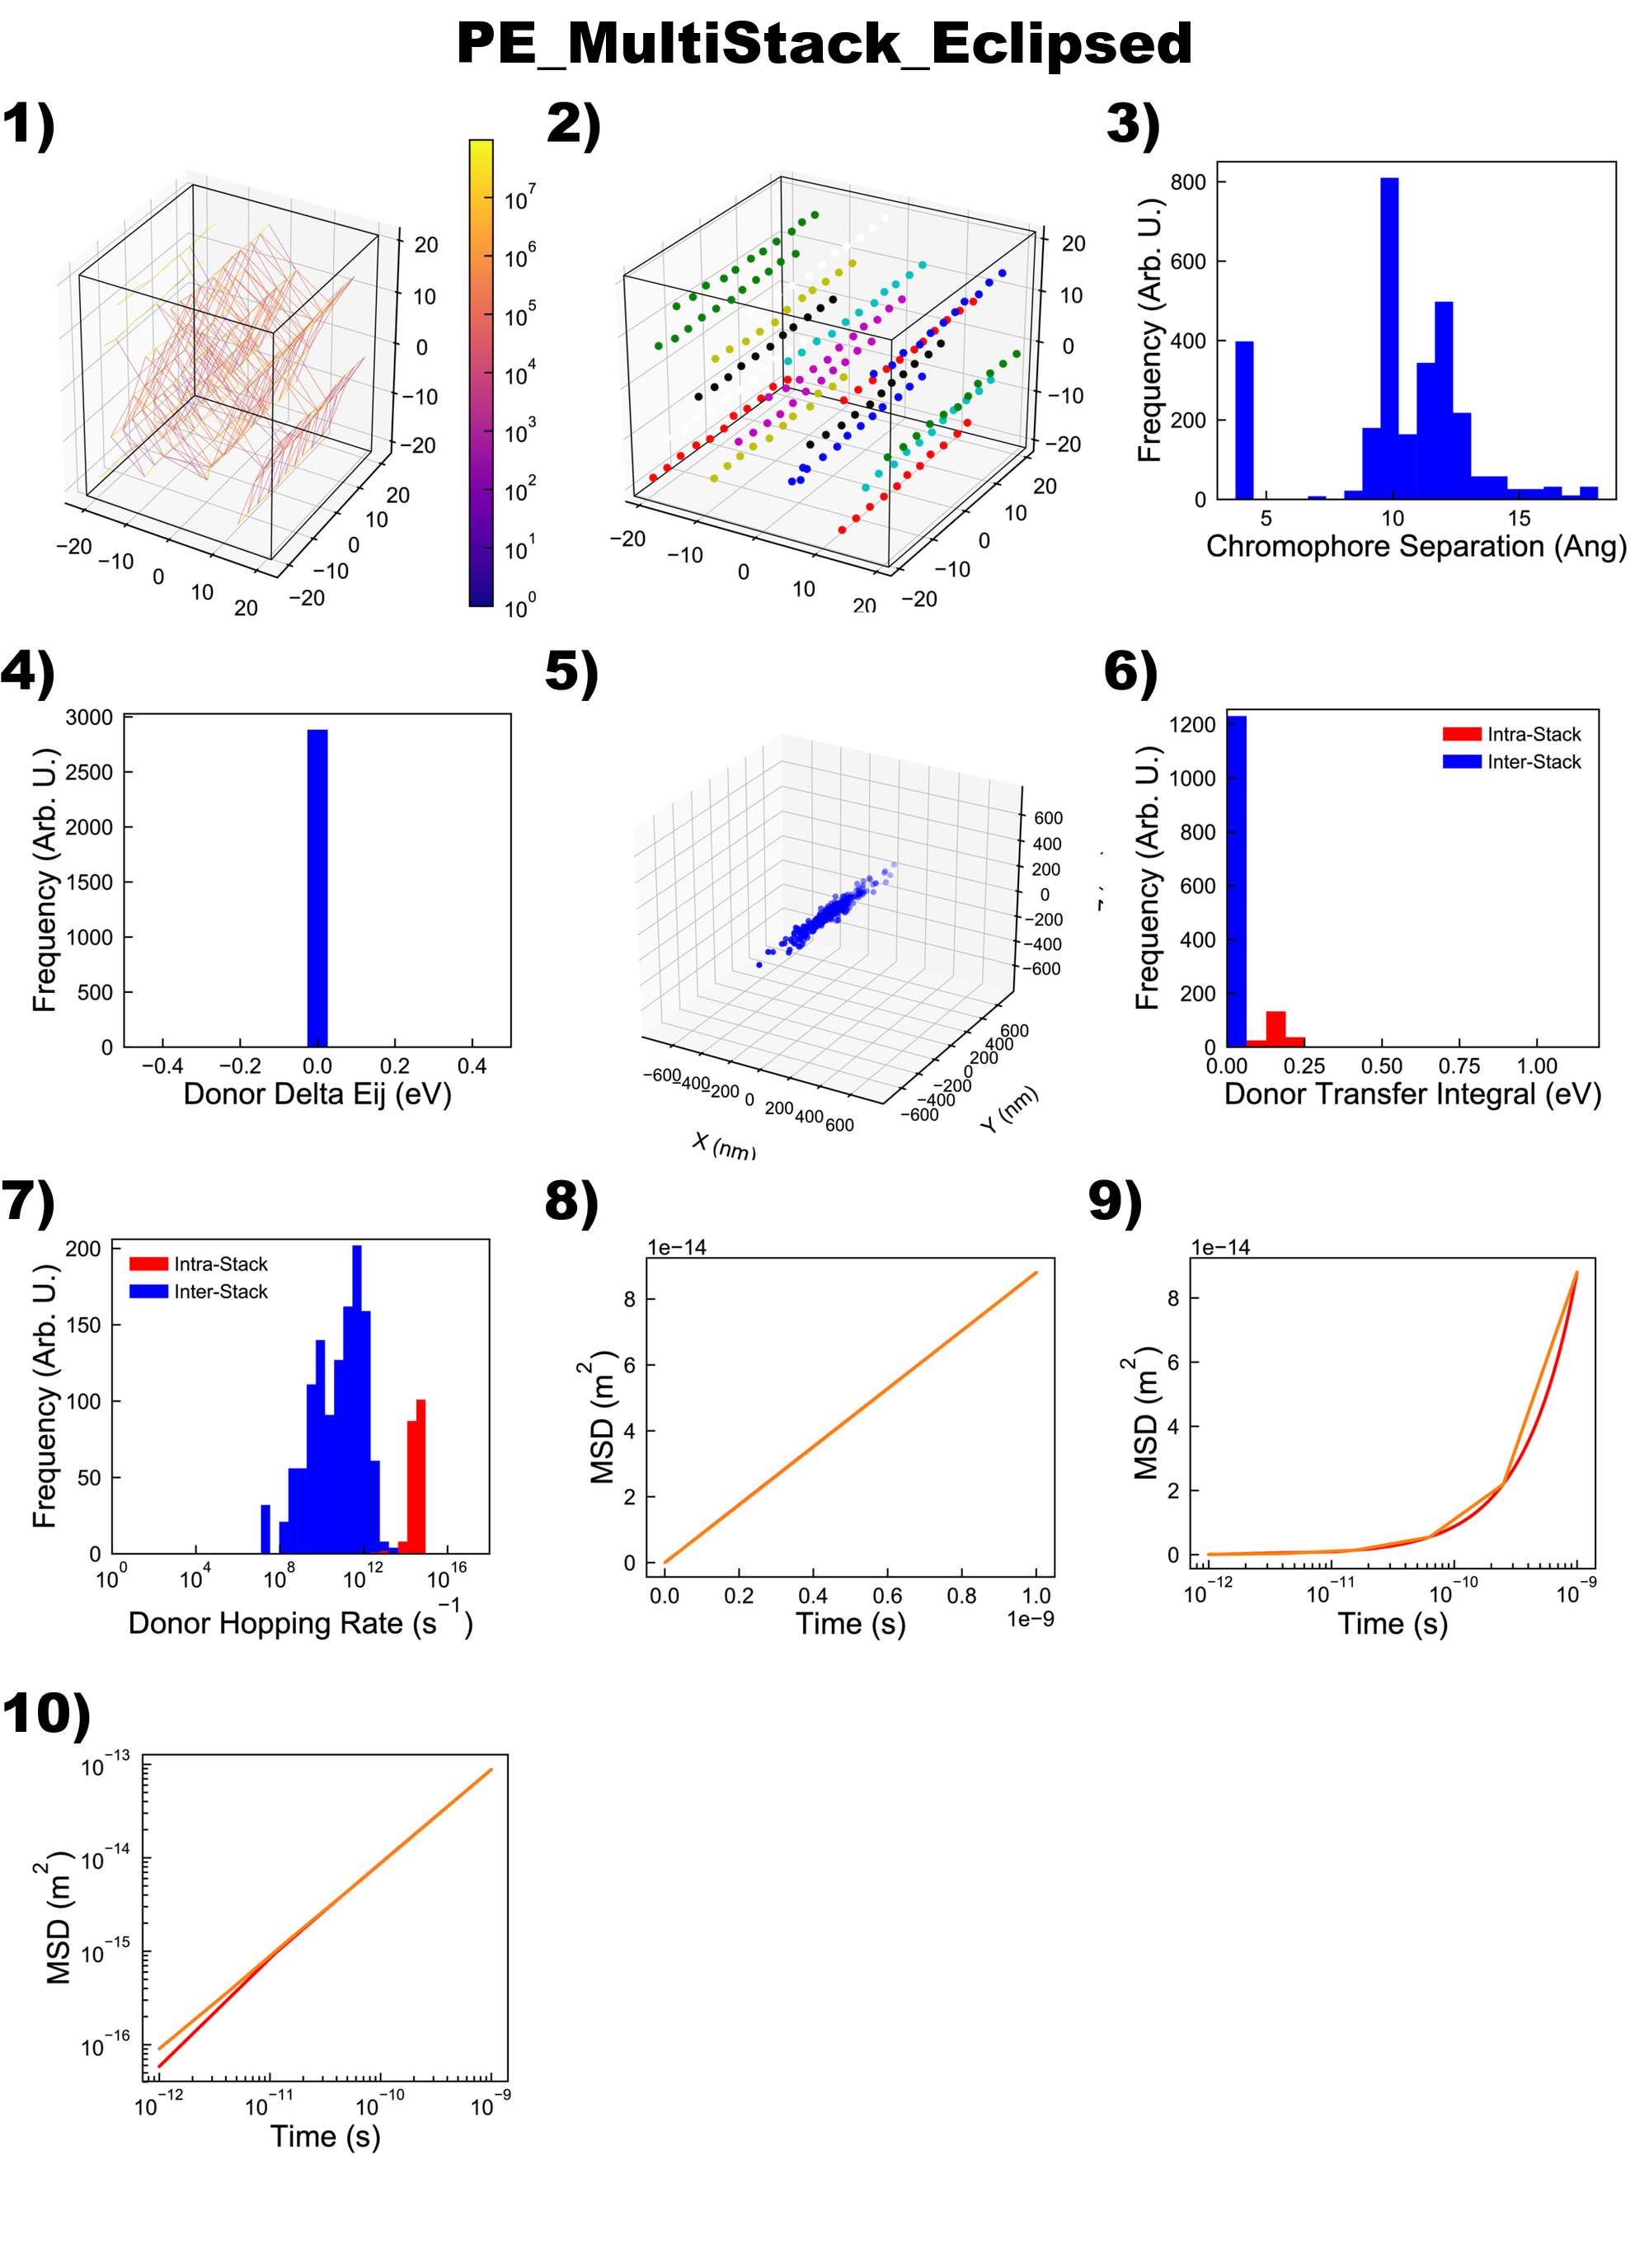
\includegraphics[width=0.85\textwidth]{Figures/PE_MultiStack_Eclipsed.png}
    \caption{   1) Chromophore connectivity network, 
                2) Location of `stacks', 
                3) Distribution of connected chromophore separations (defines stacks),
                4) Density of states of Frontier molecular orbital (delta Eij),
                5) KMC Carrier termination locations (defines anisotropy),
                6) Histogram of molecular transfer integrals,
                7) Histogram of stack transfer integrals,
                8) Histogram of molecular hopping rates,
                9) Histogram of stack hopping rates,
                10) Linear MSD plot,
                11) Semi-log-x MSD plot,
                12) Logarithmic MSD plot.}
	\label{fig:PEMultEcl}
\end{figure}


\begin{figure}[h]\centering
	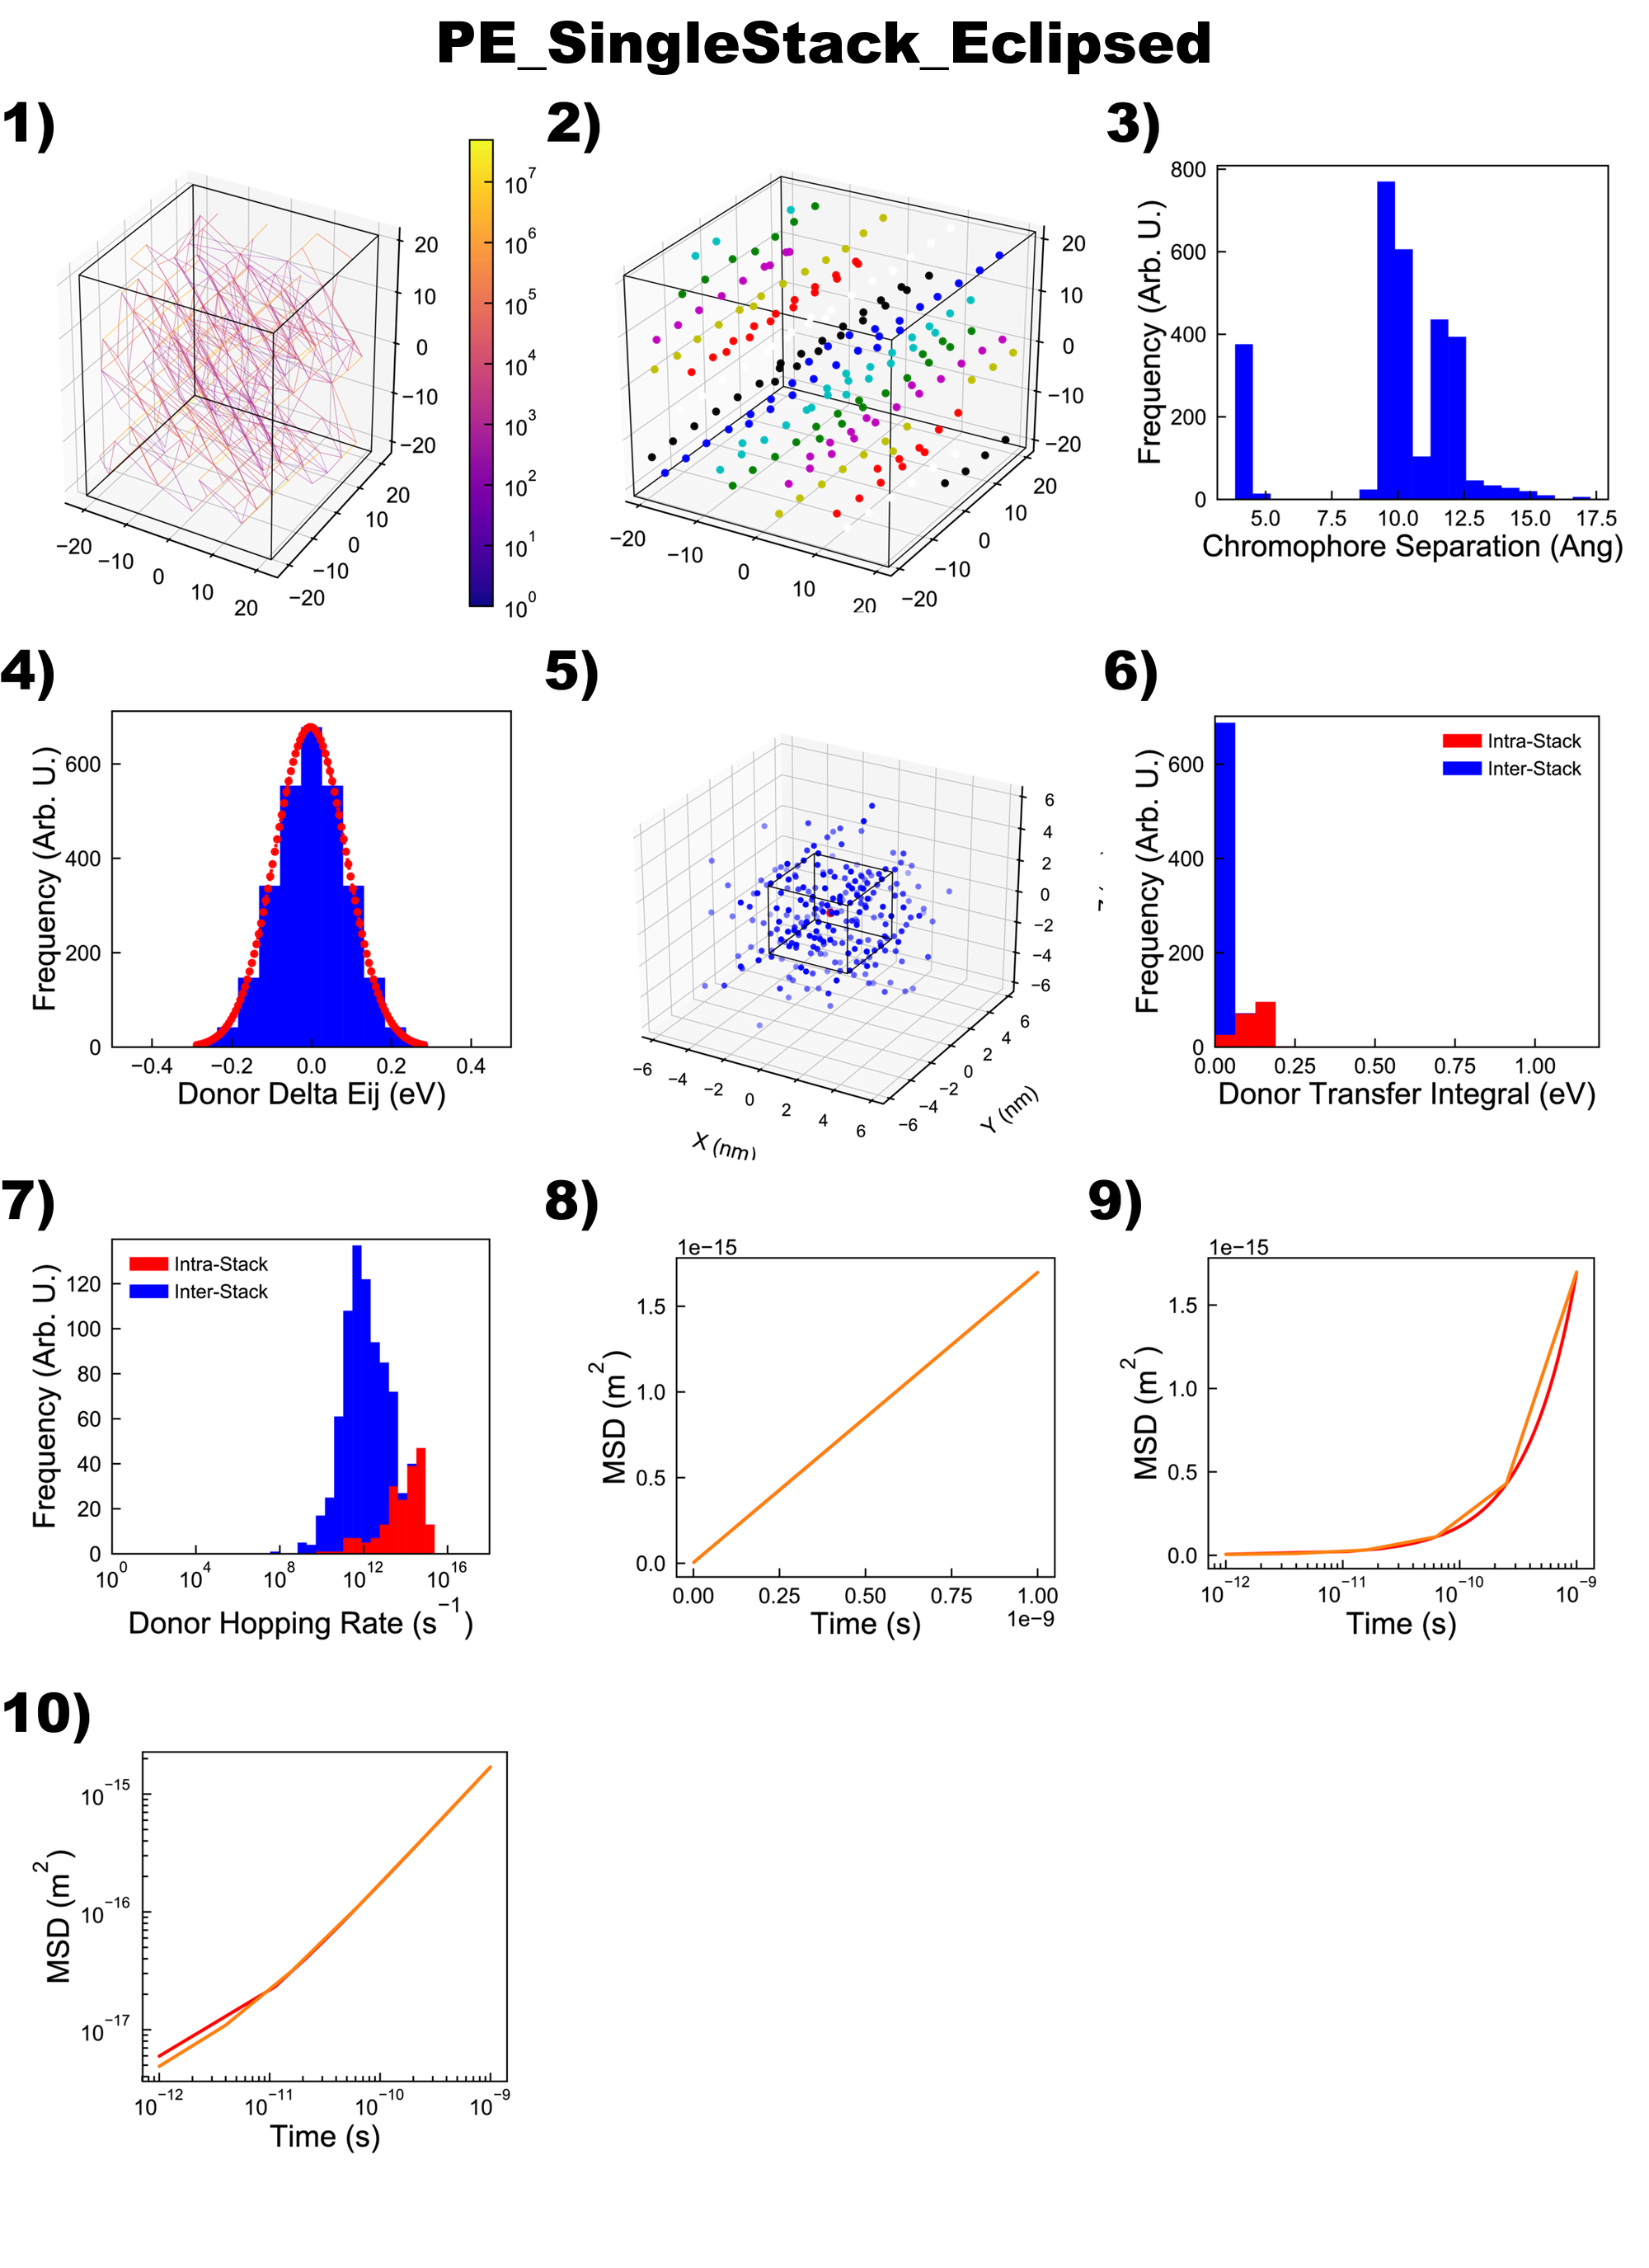
\includegraphics[width=0.85\textwidth]{Figures/PE_SingleStack_Eclipsed.png}
    \caption{   1) Chromophore connectivity network, 
                2) Location of `stacks', 
                3) Distribution of connected chromophore separations (defines stacks),
                4) Density of states of Frontier molecular orbital (delta Eij),
                5) KMC Carrier termination locations (defines anisotropy),
                6) Histogram of molecular transfer integrals,
                7) Histogram of stack transfer integrals,
                8) Histogram of molecular hopping rates,
                9) Histogram of stack hopping rates,
                10) Linear MSD plot,
                11) Semi-log-x MSD plot,
                12) Logarithmic MSD plot.}
	\label{fig:PESingEcl}
\end{figure}


\begin{figure}[h]\centering
	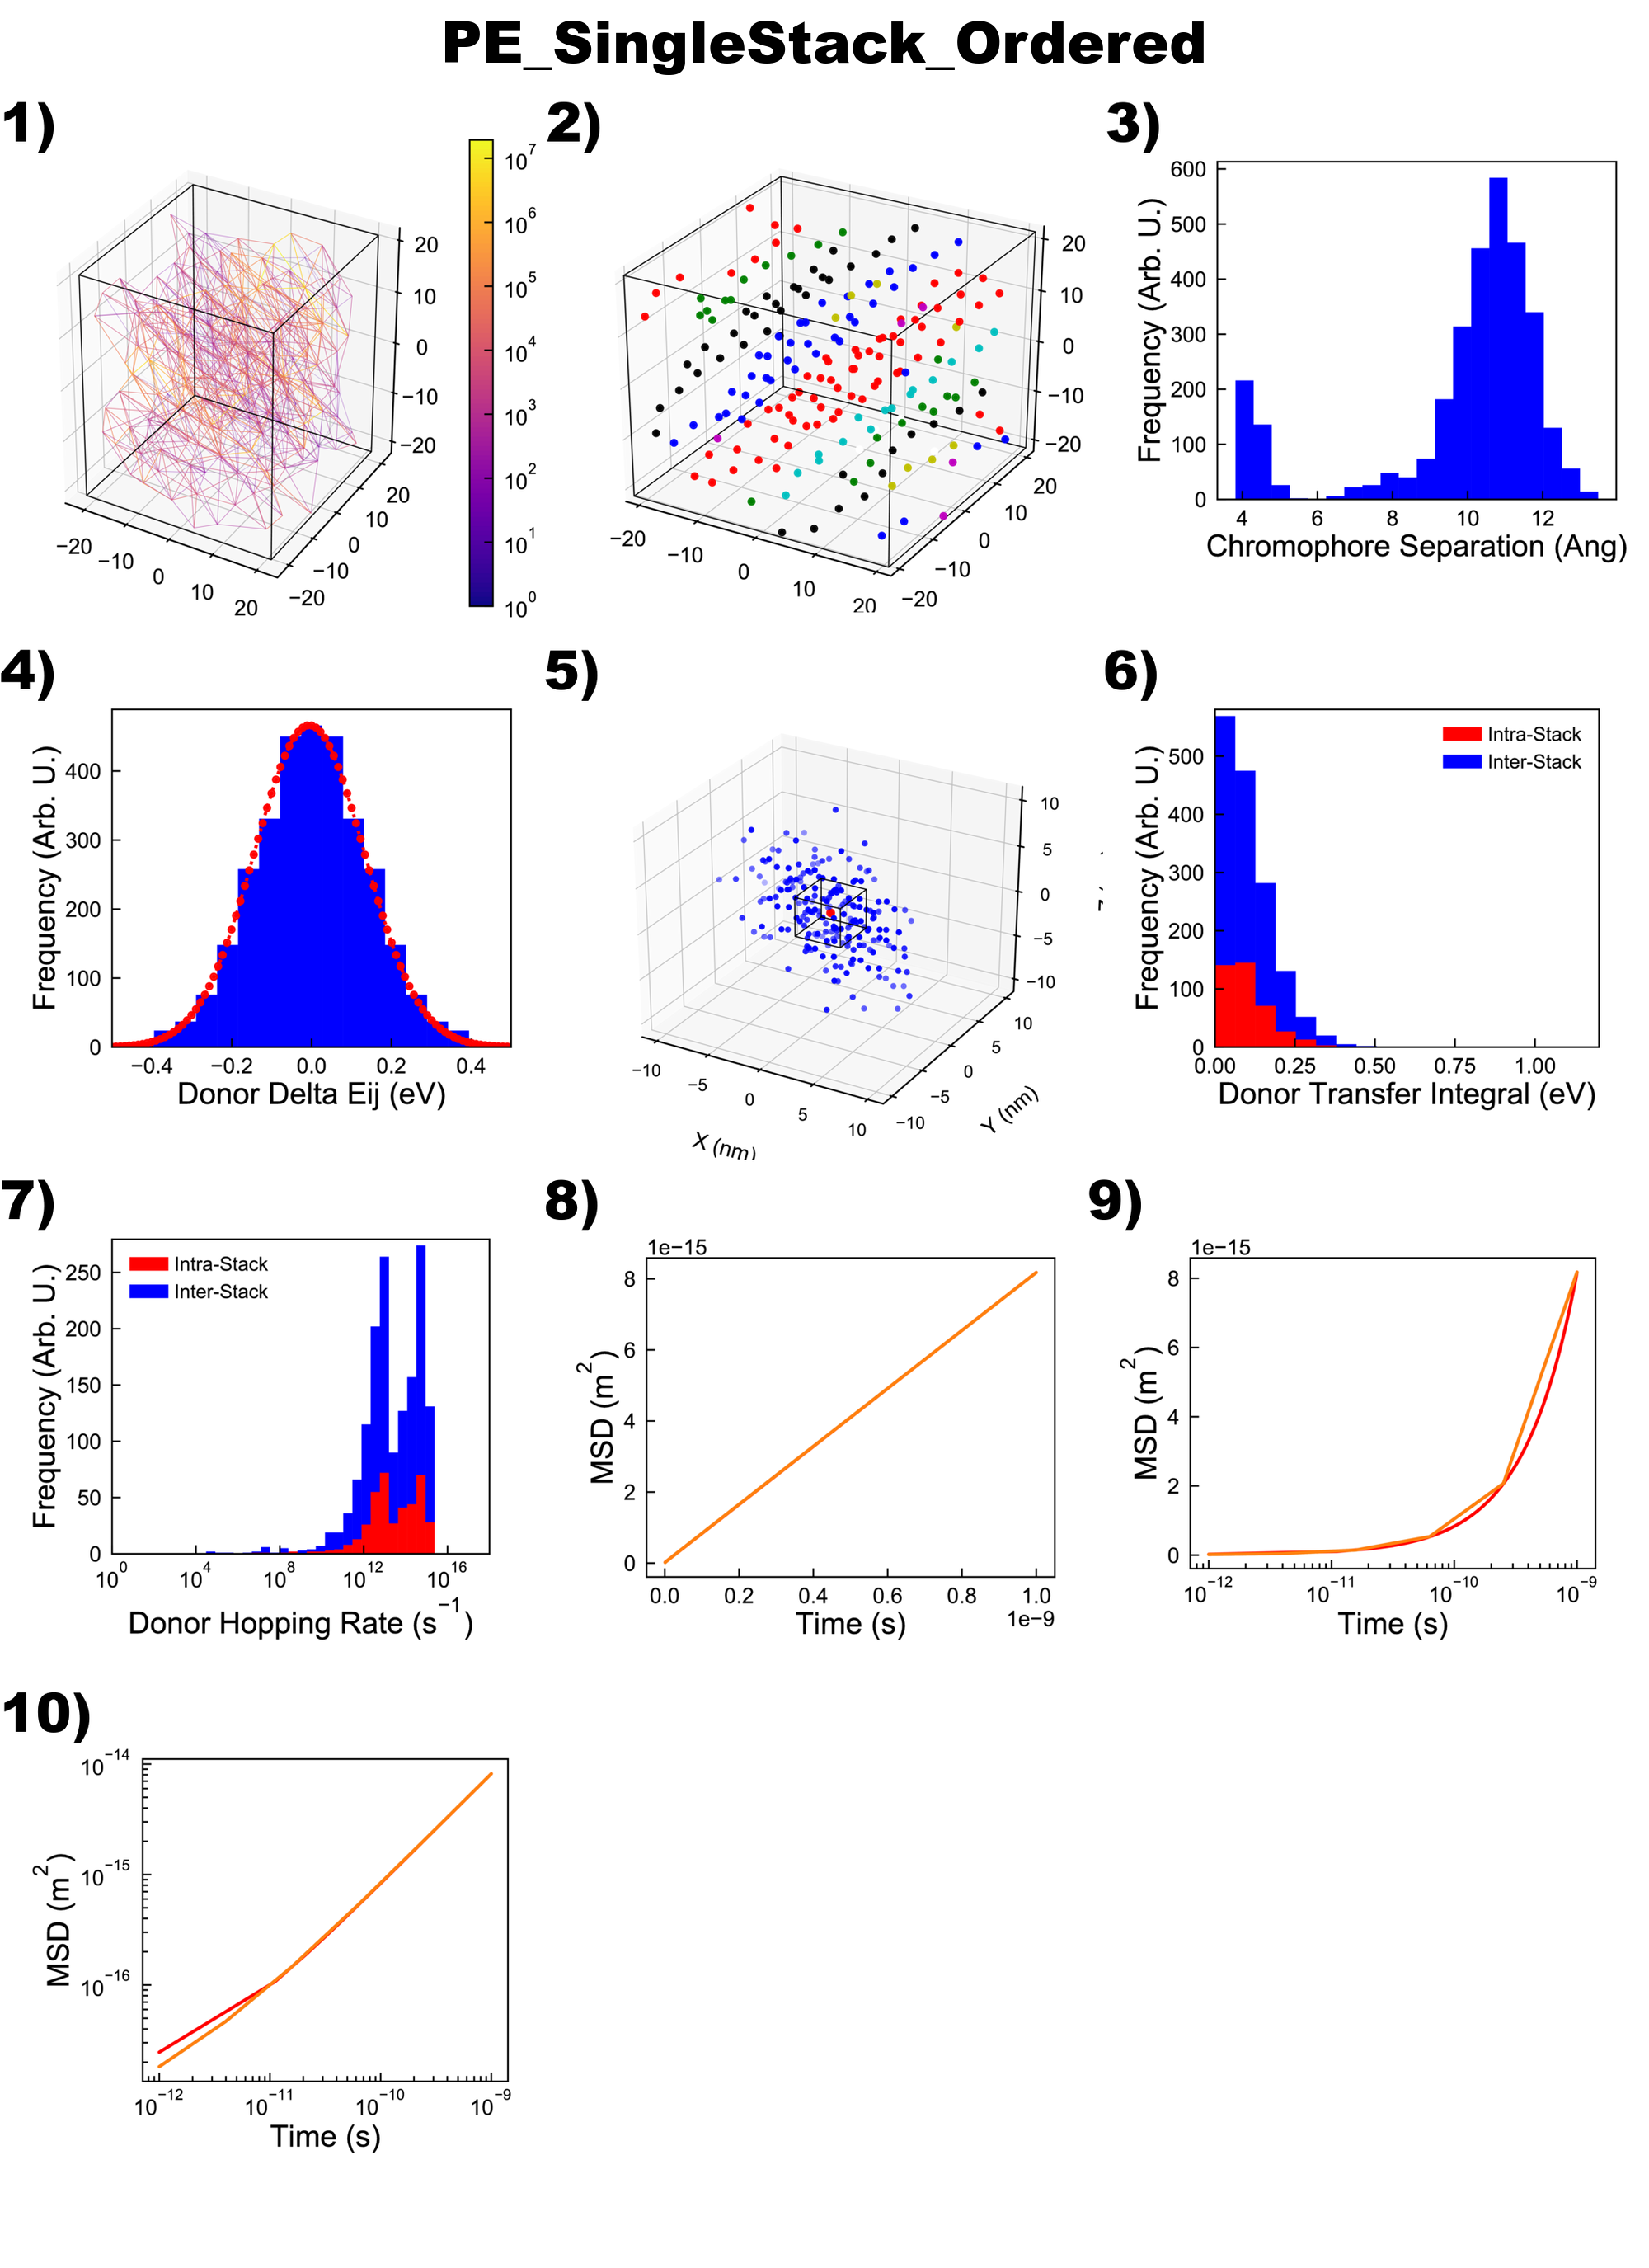
\includegraphics[width=0.85\textwidth]{Figures/PE_SingleStack_Ordered.png}
    \caption{   1) Chromophore connectivity network, 
                2) Location of `stacks', 
                3) Distribution of connected chromophore separations (defines stacks),
                4) Density of states of Frontier molecular orbital (delta Eij),
                5) KMC Carrier termination locations (defines anisotropy),
                6) Histogram of molecular transfer integrals,
                7) Histogram of stack transfer integrals,
                8) Histogram of molecular hopping rates,
                9) Histogram of stack hopping rates,
                10) Linear MSD plot,
                11) Semi-log-x MSD plot,
                12) Logarithmic MSD plot.}
	\label{fig:PESingOrd}
\end{figure}


\begin{figure}[h]\centering
	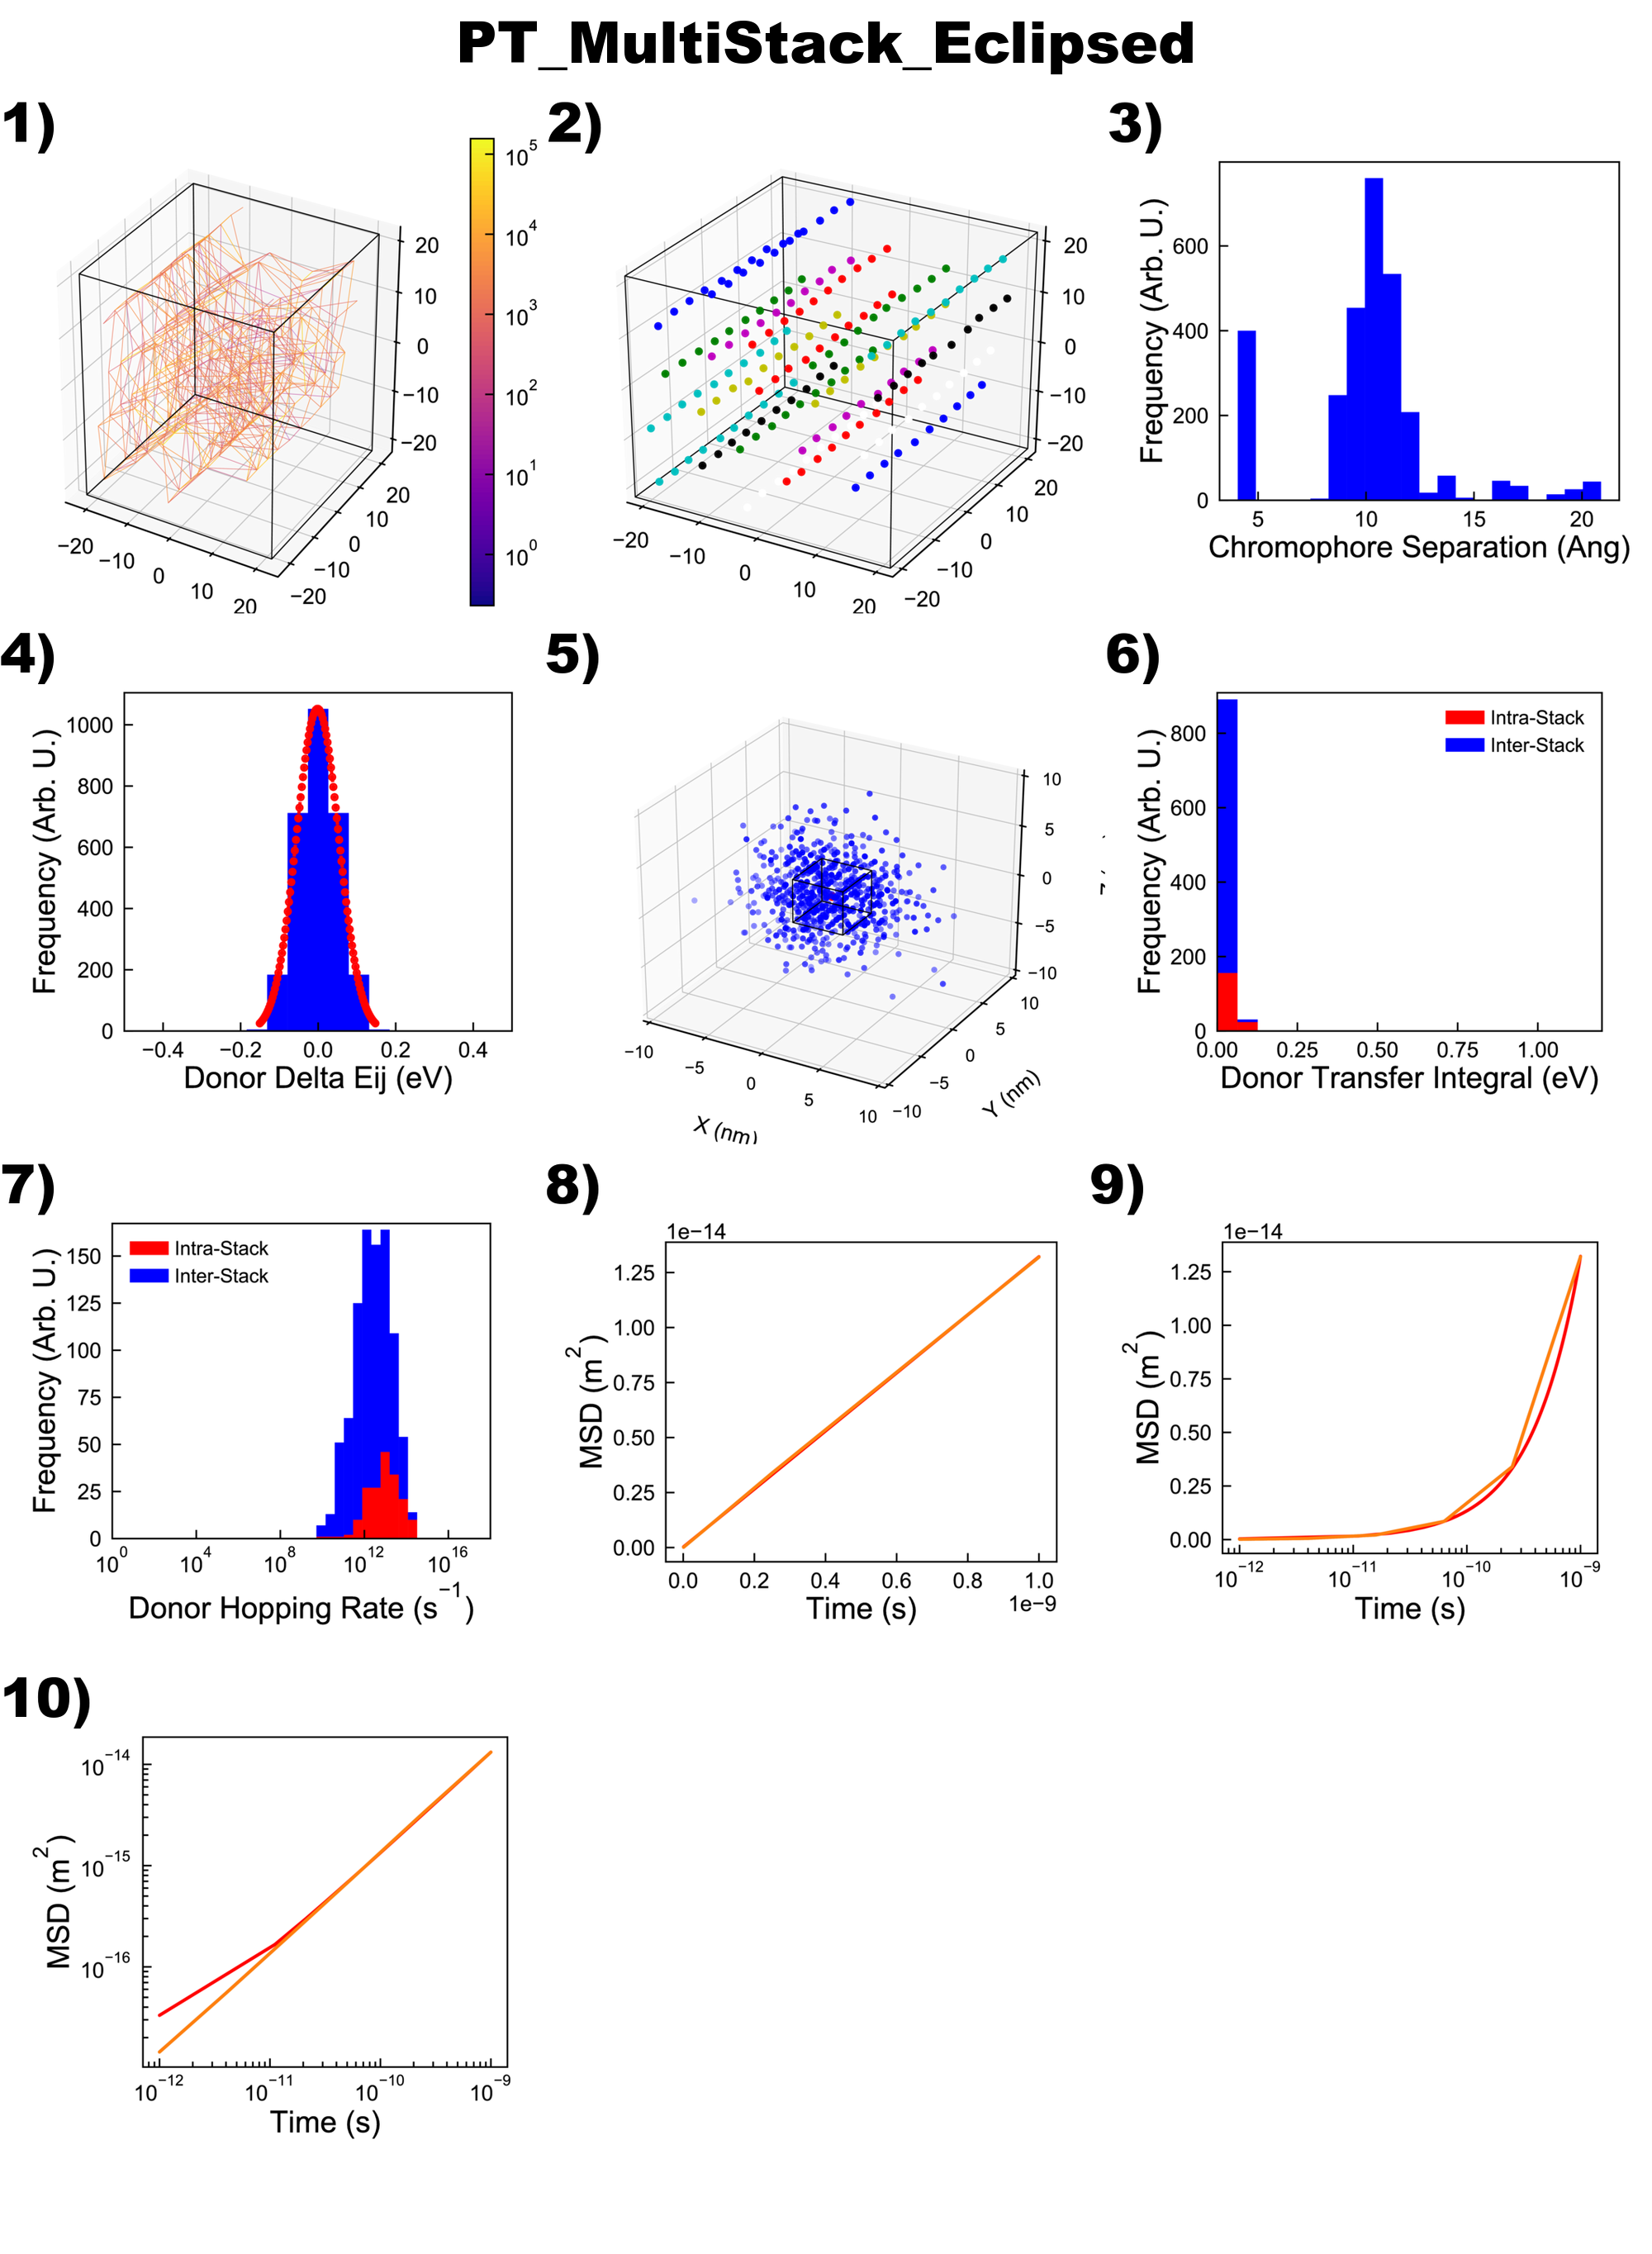
\includegraphics[width=0.85\textwidth]{Figures/PT_MultiStack_Eclipsed.png}
    \caption{   1) Chromophore connectivity network, 
                2) Location of `stacks', 
                3) Distribution of connected chromophore separations (defines stacks),
                4) Density of states of Frontier molecular orbital (delta Eij),
                5) KMC Carrier termination locations (defines anisotropy),
                6) Histogram of molecular transfer integrals,
                7) Histogram of stack transfer integrals,
                8) Histogram of molecular hopping rates,
                9) Histogram of stack hopping rates,
                10) Linear MSD plot,
                11) Semi-log-x MSD plot,
                12) Logarithmic MSD plot.}
	\label{fig:PTMultEcl}
\end{figure}


\begin{figure}[h]\centering
	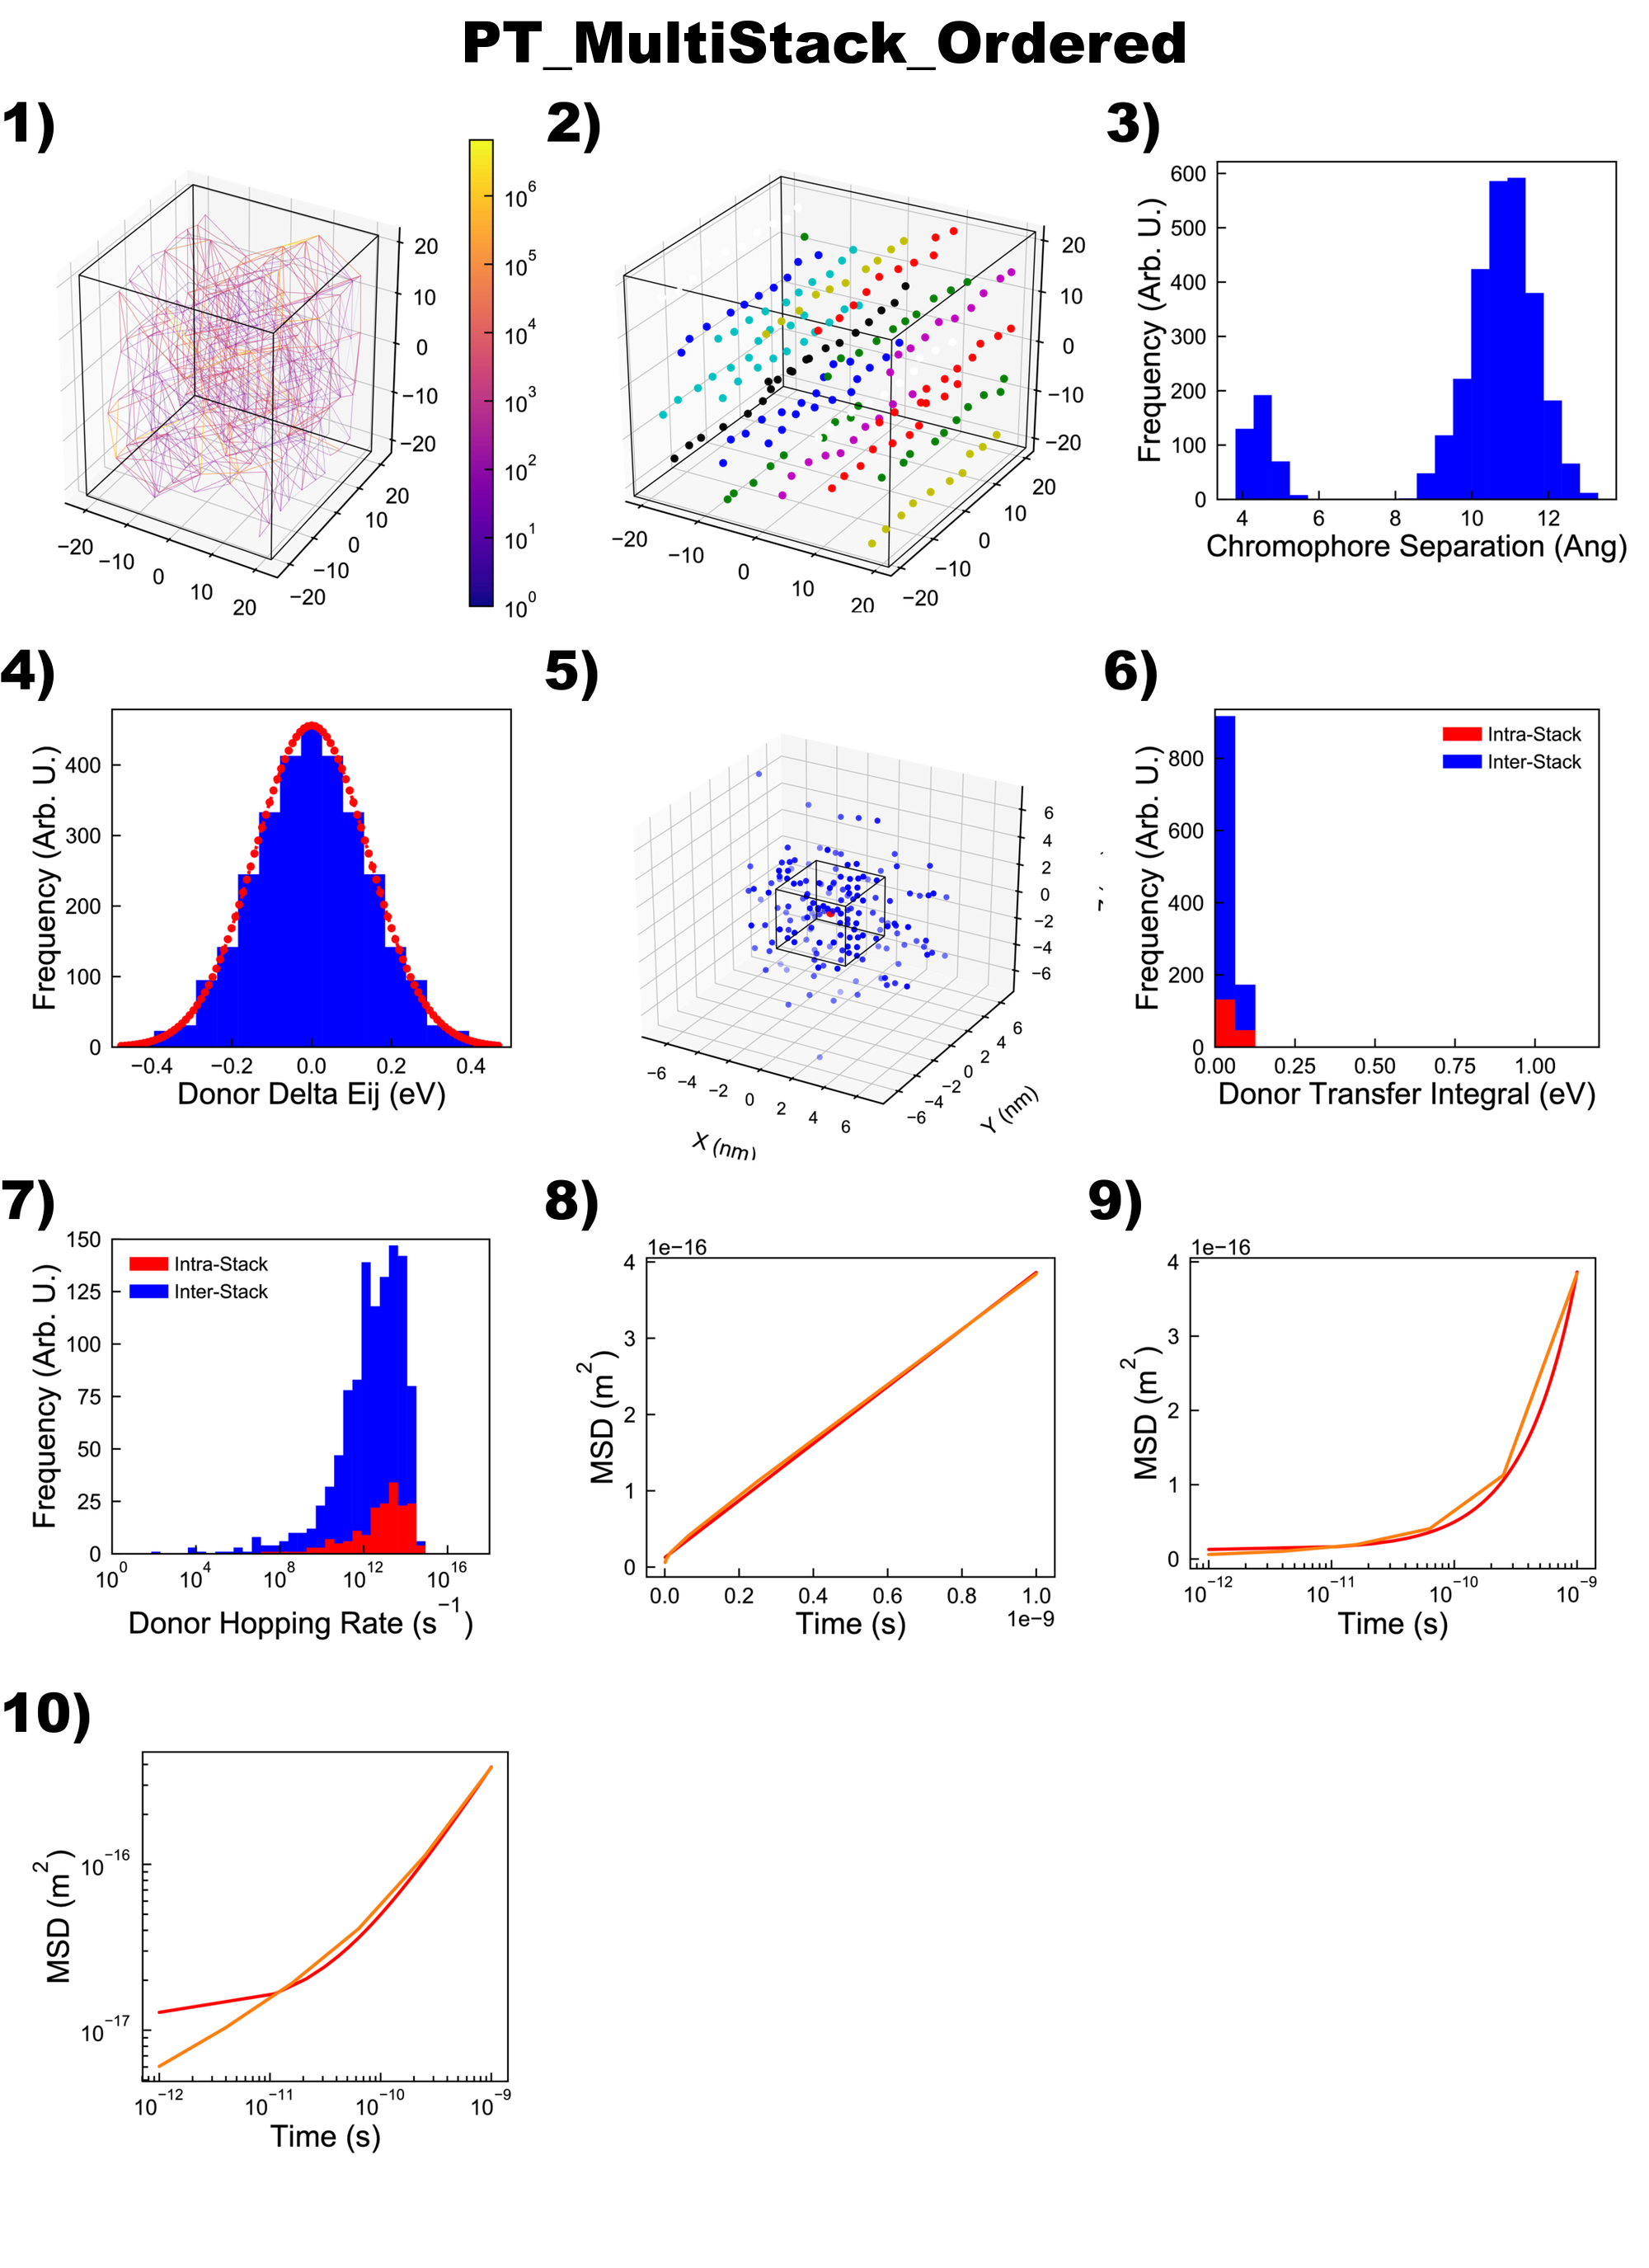
\includegraphics[width=0.85\textwidth]{Figures/PT_MultiStack_Ordered.png}
    \caption{   1) Chromophore connectivity network, 
                2) Location of `stacks', 
                3) Distribution of connected chromophore separations (defines stacks),
                4) Density of states of Frontier molecular orbital (delta Eij),
                5) KMC Carrier termination locations (defines anisotropy),
                6) Histogram of molecular transfer integrals,
                7) Histogram of stack transfer integrals,
                8) Histogram of molecular hopping rates,
                9) Histogram of stack hopping rates,
                10) Linear MSD plot,
                11) Semi-log-x MSD plot,
                12) Logarithmic MSD plot.}
	\label{fig:PTMultOrd}
\end{figure}


\begin{figure}[h]\centering
	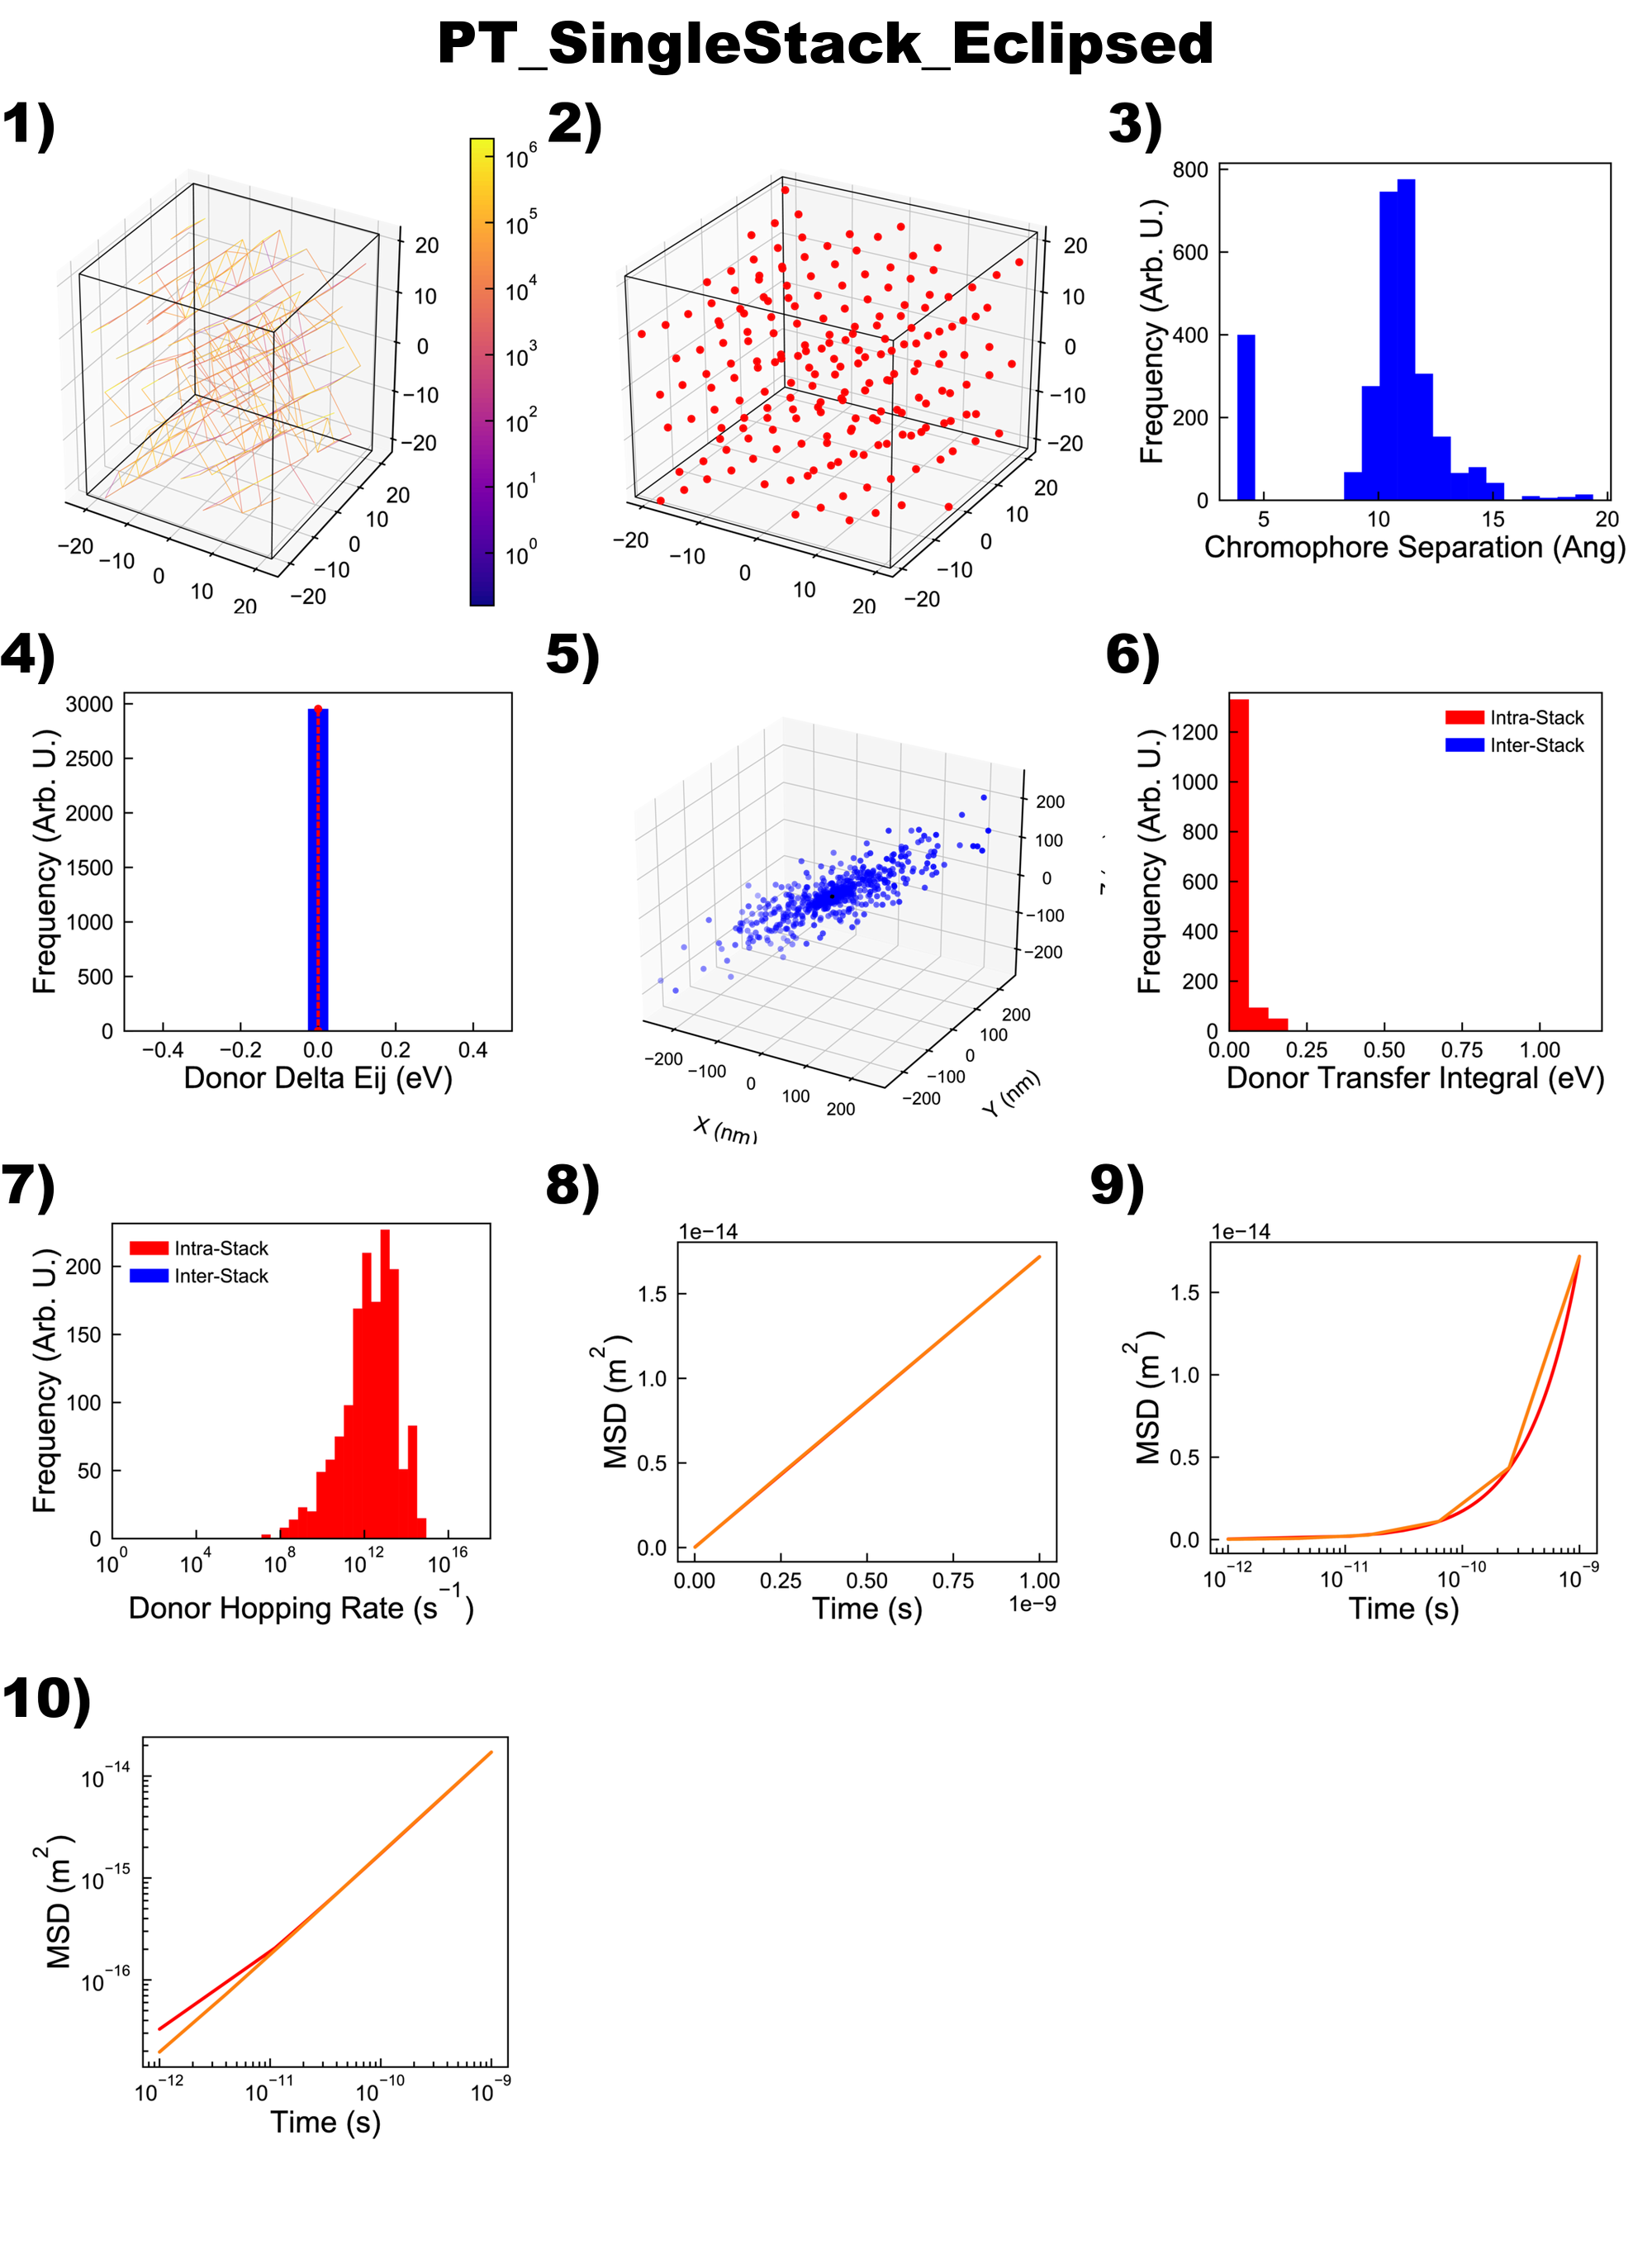
\includegraphics[width=0.85\textwidth]{Figures/PT_SingleStack_Eclipsed.png}
    \caption{   1) Chromophore connectivity network, 
                2) Location of `stacks', 
                3) Distribution of connected chromophore separations (defines stacks),
                4) Density of states of Frontier molecular orbital (delta Eij),
                5) KMC Carrier termination locations (defines anisotropy),
                6) Histogram of molecular transfer integrals,
                7) Histogram of stack transfer integrals,
                8) Histogram of molecular hopping rates,
                9) Histogram of stack hopping rates,
                10) Linear MSD plot,
                11) Semi-log-x MSD plot,
                12) Logarithmic MSD plot.}
	\label{fig:PTSingEcl}
\end{figure}


\begin{figure}[h]\centering
	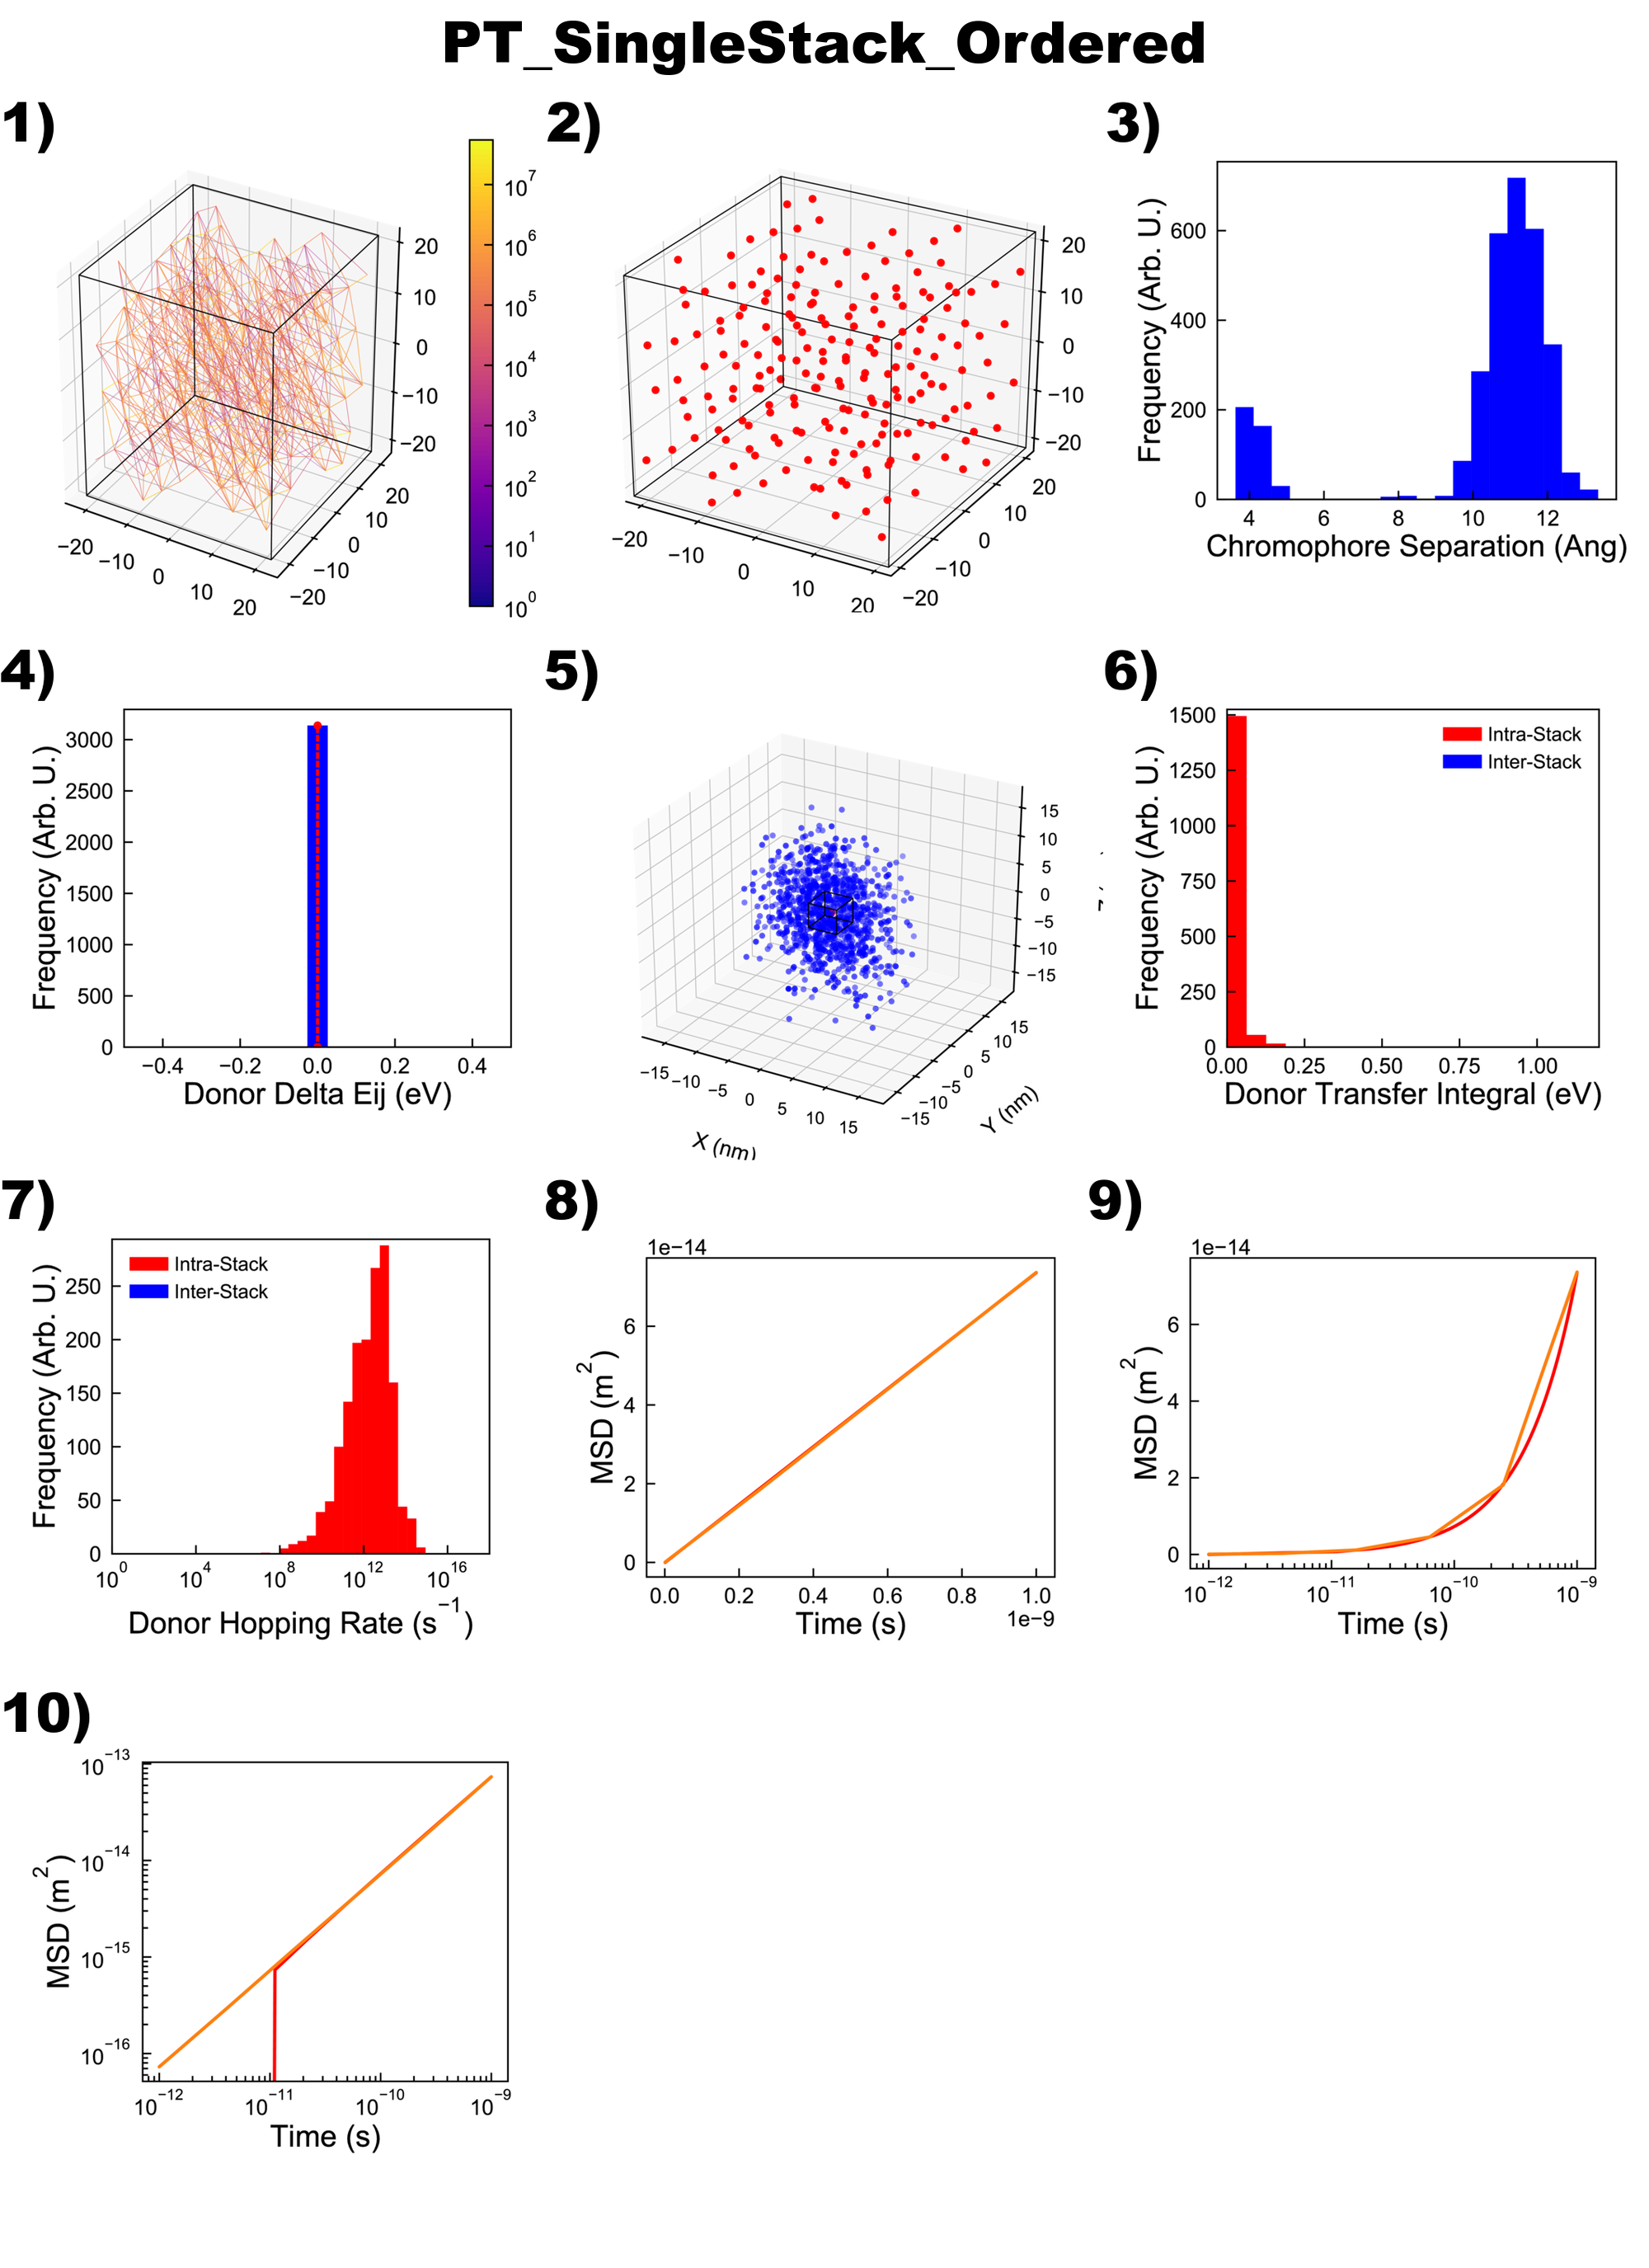
\includegraphics[width=0.85\textwidth]{Figures/PT_SingleStack_Ordered.png}
    \caption{   1) Chromophore connectivity network, 
                2) Location of `stacks', 
                3) Distribution of connected chromophore separations (defines stacks),
                4) Density of states of Frontier molecular orbital (delta Eij),
                5) KMC Carrier termination locations (defines anisotropy),
                6) Histogram of molecular transfer integrals,
                7) Histogram of stack transfer integrals,
                8) Histogram of molecular hopping rates,
                9) Histogram of stack hopping rates,
                10) Linear MSD plot,
                11) Semi-log-x MSD plot,
                12) Logarithmic MSD plot.}
	\label{fig:PTSingOrd}
\end{figure}


\subsection{Conclusions}


\begin{itemize}
    \item{Exploring the $\Delta E_{ij}$ has shown that some of the systems (namely PE\_MultiStack\_Eclipsed, PT\_SingleStack\_Eclipsed, and PE\_SingleStack\_Ordered) contain rigid bodies (delta function for the DoS), whereas others don't.
        Having a $\Delta E_{ij} = 0$ will strongly affect (increase) the eventual hopping rate and so we are comparing apples to oranges.}
    \item{Additionally, while the PT\_SingleStack systems are truly one single stack, the PE\_SingleStack systems are not.
        They certainly have fewer stacks, but they are not on massive periodic structure like in the PT\_SingleStack case, and so a direct comparison can not really be drawn there either.}
    \item{The carrier termination (anisotropy) graphs in panel \textbf{5)} show that carriers have not moved very far out of the simulation volume in the PT\_MultiStack, and PE\_SingleStack\_Eclipsed cases.
        All of the MSD fits are excellent, however, so this might not be an issue.}
    \item{All of the flexible PT\_MultiStack and PE\_SingleStack systems shown Gaussian DoSes with the maximum breadth permitted by the Gaussian map that we perform in MorphCT (which will shrink a distribution with $\sigma > 100 meV$ down to $\sigma = 100 meV$, but leave distributions with $\sigma \leq 100 meV$ alone).
        The breadth of the Ordered system is significantly greater than the Eclipsed system, in both cases.
    This makes sense - in the Eclipsed case, the molecules are azimuthally in-register and so are squeezed into planarity by the molecules closely packed around it.
This makes each molecule structurally indistinct, which manifests as an energetic indistinction and the $\Delta E_{ij} \rightarrow 0$.}
\end{itemize}


I think there are too many variables here that we are unable to resolve with just these 7 simulations.
This makes it impossible to draw any conclusions about the presence and orientation of the stacks other than \textcolor{blue}{``it matters and can affect the mobilities by an order of magnitude''}.
Given the strict mathematical constraints on how the stacks can form and still produce a coherent structure without morphological defects, I am not convinced that this is something we can adjust our mobilities for either.
Instead, I think it's something that we just have to be aware of when submitting our simulations to KMC, consider when drawing conclusions, and disclose fully when we present results.


%\section{New Jobs, 08/17}
%
%\begin{itemize}
%    \item{One way around the issues we've been seeing is to run larger simulations that have multiple crystallites in them.
%        The intention is to avoid problems with generating one single crystal, and the issues associated with defects arising from the periodic structure by just having a much larger simulation volume to do everything in.}
%    \item{To this end, I am currently running a 5,000 molecule (100,000 atom) system of perylene called \textit{PE-dt0.001-n\_mol5000-phi1.15-P1-T11.0}.}
%    \item{This statepoint has been selected in order to approximate experimental densities (phi 1.15) and a temperature at which we expect the system to be ordered (T < 13.0).}
%    \item{I actually ran simulations that were T = 13, 12, and 11, but all of them demonstrated a constant potential energy evolution and, while some crystallites were observed in the system, there didn't seem to be signficant order after 48 hours.}
%    \item{Now, I am taking the T = 11 system, and dropping it down to T = 9 to run for 96 hours. This will hopefully be sufficiently cold and long enough for the system to form a more ordered structure with multiple, ordered crystallites.}
%    \item{The data will be reported here when I have it.}
%\end{itemize}
%
%\newpage
%
%
%\section{Outstanding Questions}
%
%\textcolor{red}{The main questions we've tried to answer here are:
%    \begin{itemize}
%        \item{To what extent do our mobilities depend on the orientation of the periodic image? If we take the same molecular structure and rotate it such that the axis that the molecules stack along is different, do we get a different result?}
%        \item{Can we quantify that mobility trend in order to adjust for the rotation of the periodic box, and remove or at least reduce the mobility's sensitivity on it?}
%    \end{itemize}
%}
%
%\textcolor{blue}{I can't shake the feeling that this problem is too complex to adjust for.
%    We need to adjust for it because if we take the same morphology and then rotate it, we don't want to get different performance characteristics.
%    I think the only option might be to limit our KMC to just one periodic volume and calculate the mobilities from there.
%    That's going to require a bit of a rework of the mobility calculations though - we can't just run a carrier for X time if we do that, we'll need to get a bunch of t and disp data and then bin it to get the MSD trend.}
%
%\clearpage
%
%\section{Mobility Results}
%
%
%\begin{center}
%\begin{tabular}{| c | c | c | c | c | c | c |}
%\hline
%\rule{0pt}{2.5ex} 
%\multirow{2}{*}{\textbf{ID}}&\multirow{2}{*}{\textbf{Simulation Name}}&\textbf{Density}&\textbf{Anisotropy}&\textbf{Anisotropy}&\textbf{Stacks}&\textbf{Mobility}\\
%                            &&(\SI{}{\gcm})&(Arb. U.)&(Shape)&(Arb. U.)&(\SI{}{\mobunits})\\
%\hhline{|=======|}
%\textbf{\ccg1}&\rule{0pt}{2.5ex}\ccg PE\_MultiStack\_Eclipsed&\ccg 1.06&\ccg 0.9456&\ccg Thin Tube&\ccg19&\ccg5.87$\times 10^{0}$\\
%\textbf{2}&\rule{0pt}{2.5ex}PE\_SingleStack\_Eclipsed&1.06&0.2016&Fat Tube&8&$4.73\times 10^{-2}$\\
%\textbf{\ccg3}&\rule{0pt}{2.5ex}\ccg PE\_SingleStack\_Ordered&\ccg 1.06&\ccg 0.0844&\ccg Oblate Spheroid&\ccg10&\ccg5.09$\times 10^{-2}$\\
%\hhline{|=======|}
%\textbf{4}&\rule{0pt}{2.5ex}PT\_MultiStack\_Eclipsed&1.01&0.1245&Oblate Spheroid&20&2.48$\times 10^{-1}$\\
%\textbf{\ccg5}&\rule{0pt}{2.5ex}\ccg PT\_MultiStack\_Ordered&\ccg 1.01&\ccg 0.1313&\ccg Oblate Spheroid&\ccg20&\ccg1.65$\times 10^{-3}$\\
%\textbf{6}&\rule{0pt}{2.5ex}PT\_SingleStack\_Eclipsed&1.01&0.7264&Thin Tube&1&1.15$\times 10^{0}$\\
%\textbf{\ccg7}&\rule{0pt}{2.5ex}\ccg PT\_SingleStack\_Ordered&\ccg 1.01&\ccg 0.2536&\ccg Oblate Spheroid&\ccg1&\ccg2.04$\times 10^{-1}$\\
%\hhline{-------}
%\end{tabular}\label{table:mob}
%\captionof{table}{The results from MorphCT for the various PAH morphologies. See the below section for a discussion of the stacks.}
%\end{center}
%
%Representative Values From Literature:
%\begin{itemize}
%    \item{PE Mobility: 2E-1 (one paper reports 5E2)}
%    \item{PT Mobility: 8E-1}
%\end{itemize}
%
%Comments:
%\begin{itemize}
%    \item{The mobilities reported here vary significantly, but generally have good experimental agreeement}
%    \item{As expected, the eclipsed systems \textbf{1}, \textbf{2} and \textbf{6} generally have higher anisotropies than their comparable ordered systems.
%        This is due to a higher degree of order along the stack, which makes it easier for carriers to travel along the stack, resulting in more anisotropic transport.}
%    \item{However, this trend is only the case for the single-stack systems, where the columns pack off the simulation volume axes.
%        This means, due to periodic boundary conditions, that the simulation volume actually only contains a single stack as carriers can `hop to adjacent stacks' by simply continuing along the current one.}
%    \item{The discrepancy between the off-axis single-stack systems (\textbf{2}, \textbf{3}, \textbf{6}) and the along-axis multiple-stack systems (\textbf{1}, \textbf{4}, \textbf{5}) is visible in the comparisons of the perylothiophene systems.
%            \begin{itemize}
%                \item{Anisotropy is significantly lower in the eclipsed case (\textbf{4} compared to \textbf{6}) when multiple stacks are present, compared to a single stack.
%                    This could partially be a result of the slight herringbone structure observed in the multiple-stack systems increasing the transfer integrals to neighbouring stacks, permitting more parity between transport along- and between-stacks.}
%                \item{Mobility is also lessened by at least an order of magnitude.
%                    This again could result from the herringbone structure which forces neighbouring molecules within a stack slightly further apart to accomodate the alternating orientations of molecules between stacks.}
%            \end{itemize}
%        }
%    \item{The perylene systems \textbf{1} and \textbf{2} do not exhibit the above behaviour - the mobility trend is reversed (the single-stack mobility in \textbf{2} is two orders of magnitude slower than the multi-stack mobility of \textbf{1}).
%            This reinforces the idea that the difference between the single- and multi-stack cases is a factor of the herringbone-like packing observed in perylothiophene, as the perylene systems do not exhibit the same herringbone-like structure.
%        \textcolor{red}{What is the reason for the two order of magnitude discrepancy in the mobility then, if neither system exhibits herringbone packing?}}
%\end{itemize}
%
%\clearpage
%
%\subsection{3D Carrier Network}
%
%\begin{figure}[h!]\centering
%	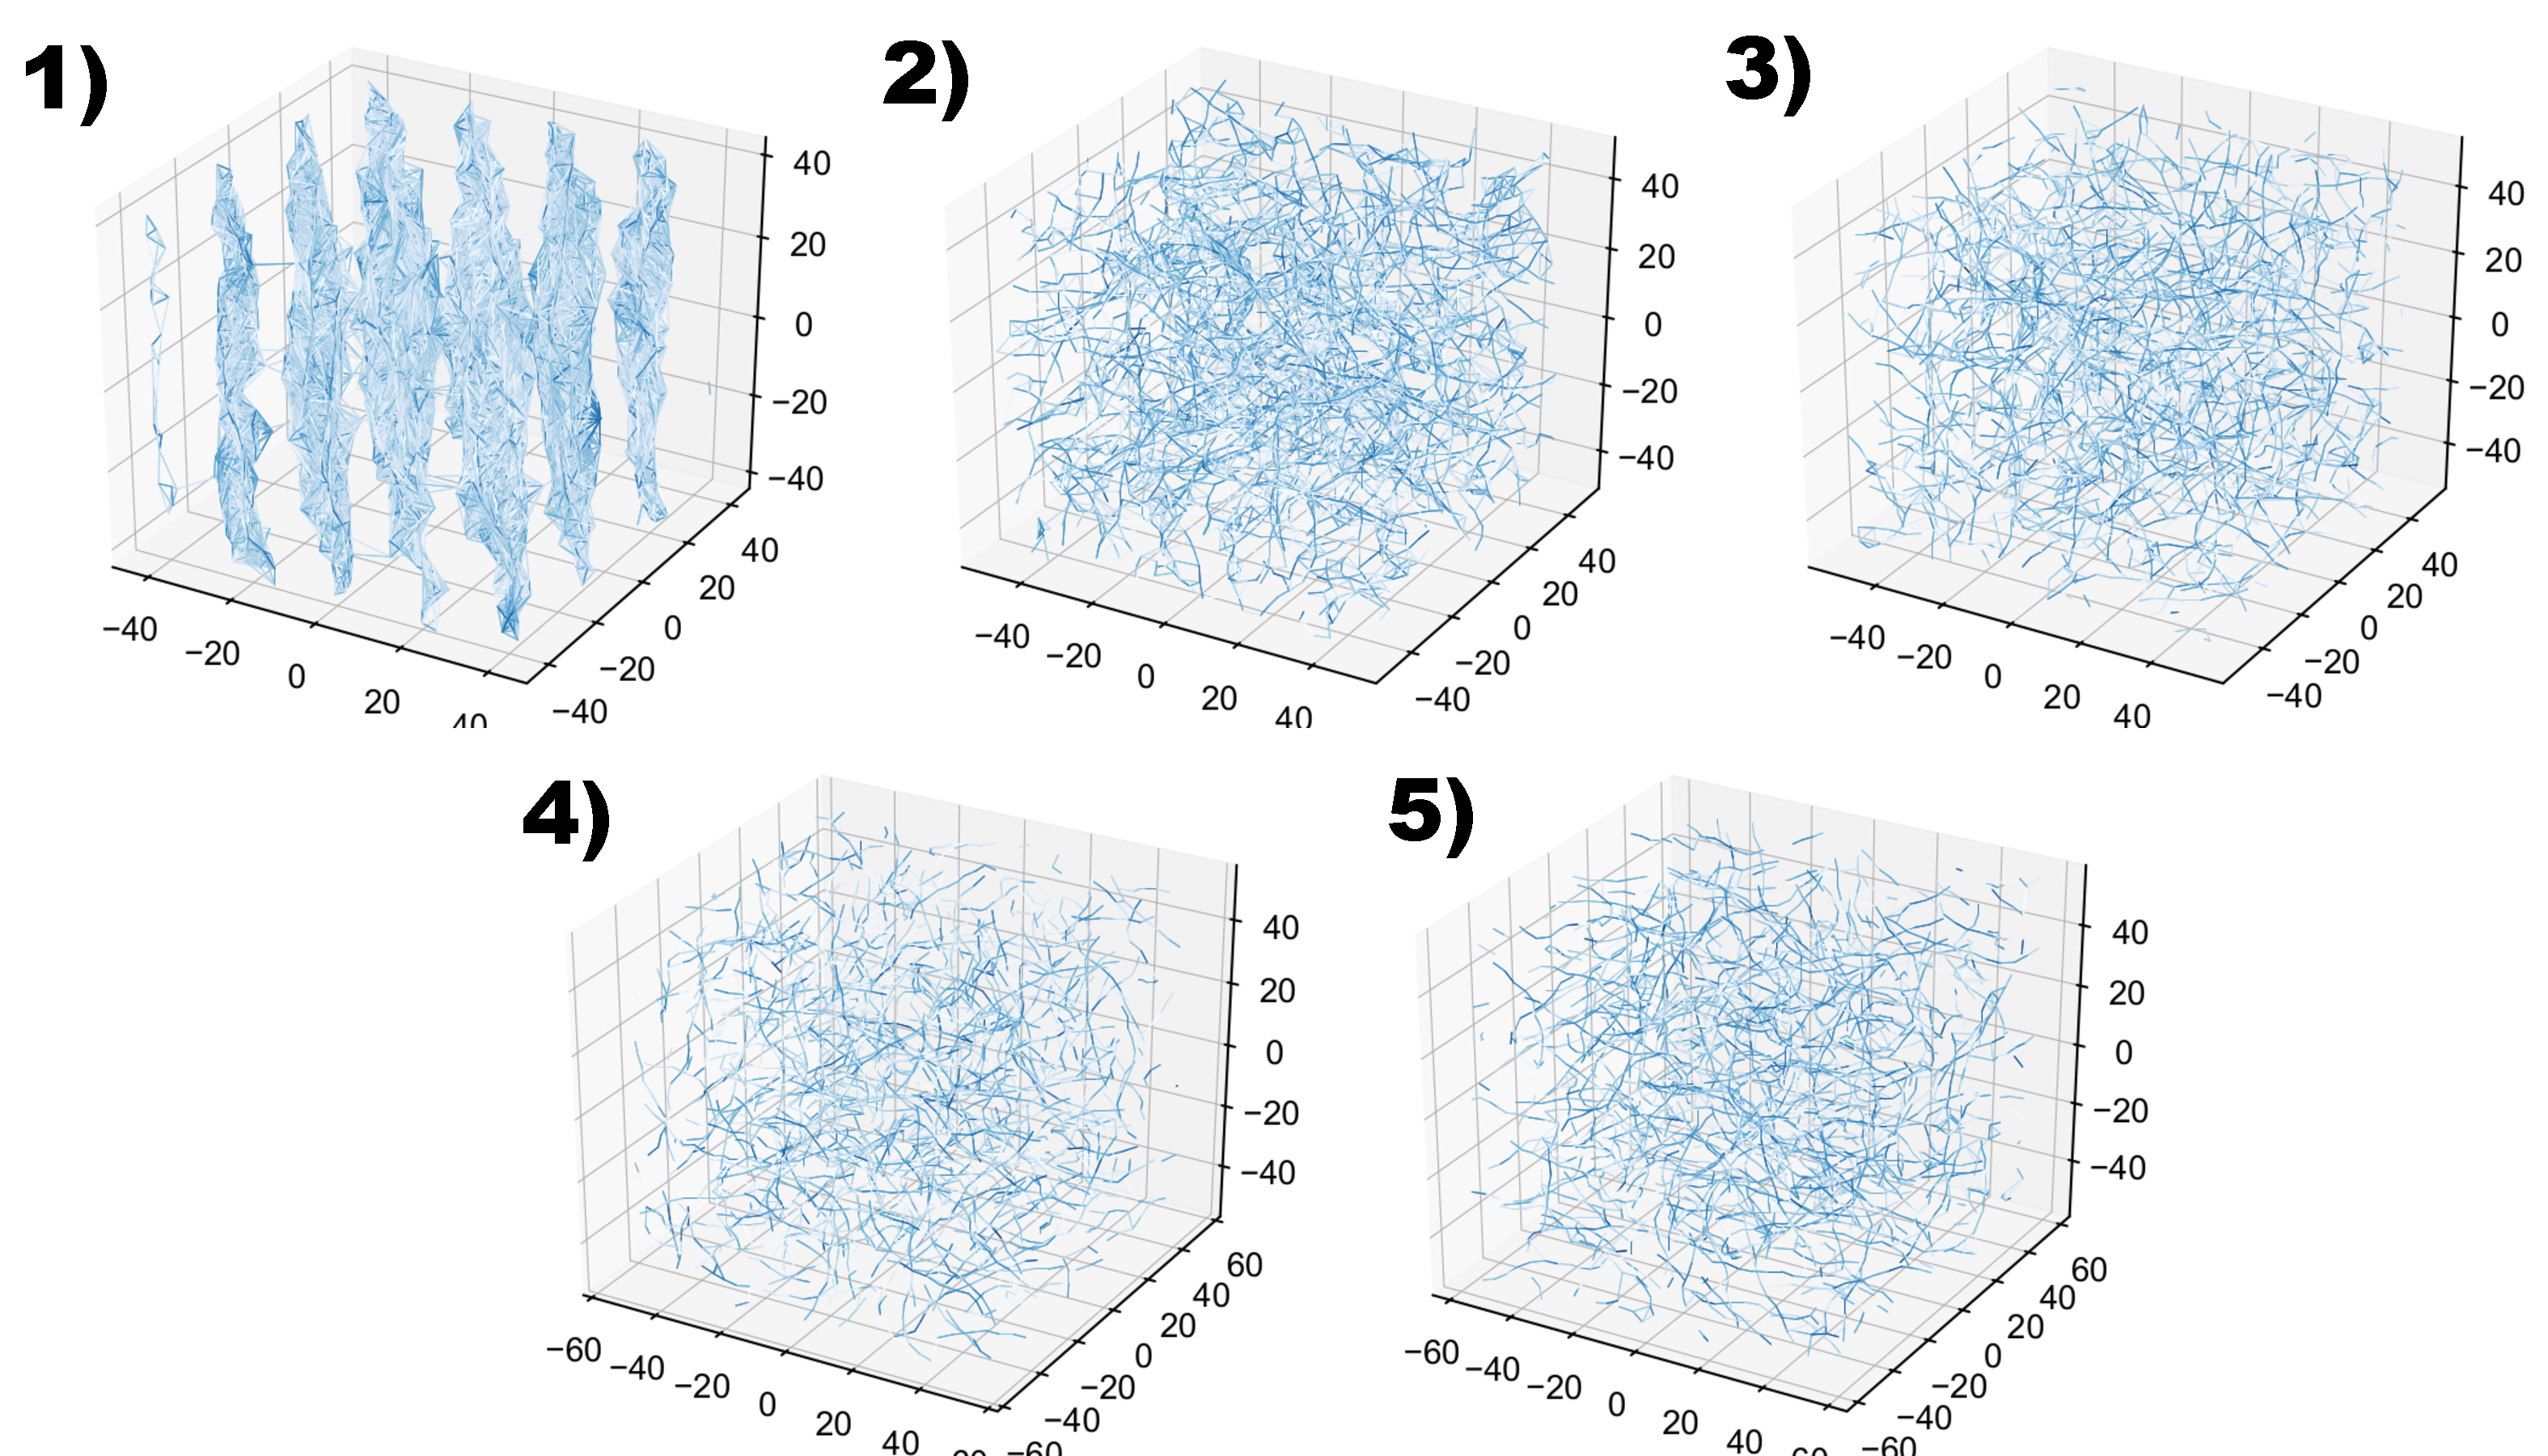
\includegraphics[width=\textwidth]{Figures/3dHole.pdf}
%    \caption{The 3D heatmap of charge transport routes within the morphologies \textbf{1} - \textbf{7}.
%    Dark routes describe commonly accessed hops between pairs of chromophores, whereas pale routes are less widely used in the KMC simulations.
%    Each node therefore represents the location of a single chromophore.
%The intensity value for the route is currently taken to be \texttt{I $=$ np.log10(freq) $/$ np.log10(max\_freq)}.}
%	\label{fig:3dNetwork}
%\end{figure}
%
%\clearpage
%
%\subsection{MSDs}
%
%\begin{figure}[h!]\centering
%	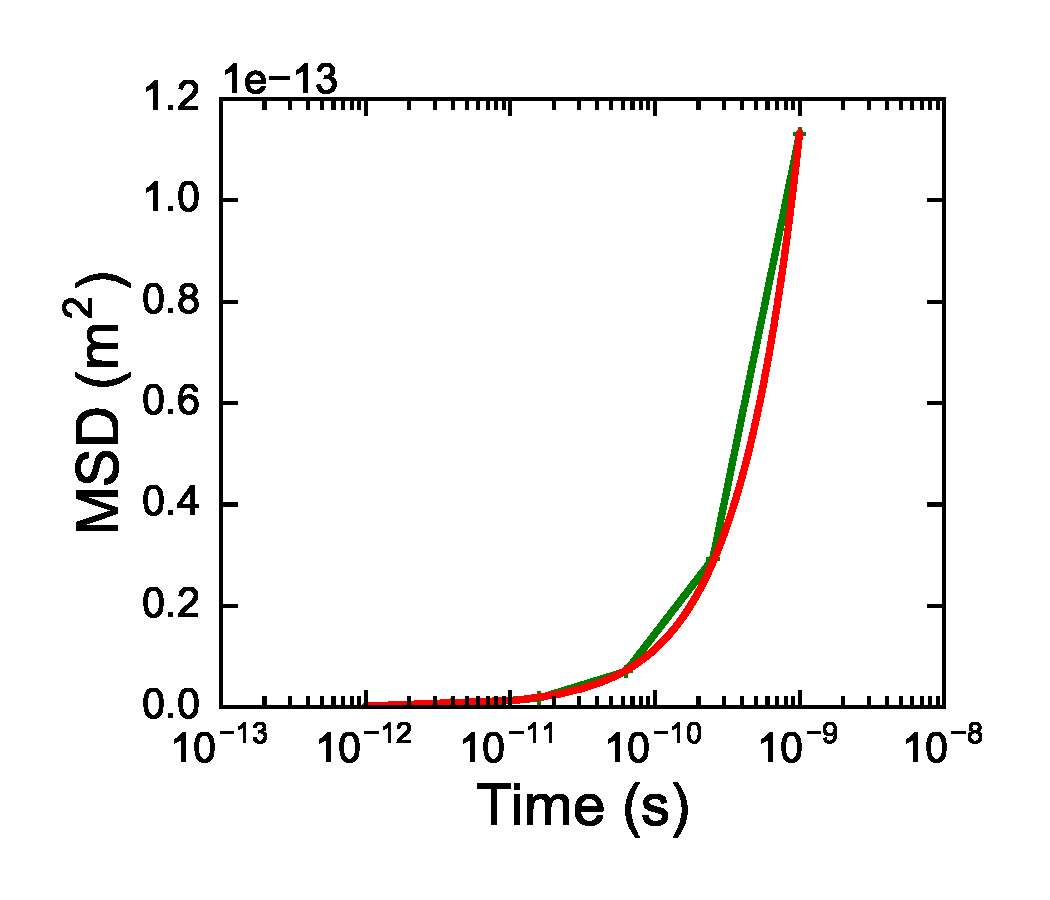
\includegraphics[width=\textwidth]{Figures/SemiLogMSDHole.pdf}
%    \caption{The semi-log-x mean squared displacement curves of the carriers within the morphologies \textbf{1} - \textbf{7}.}
%	\label{fig:MSD}
%\end{figure}
%
%\begin{itemize}
%    \item{These are among the best fits we've ever had with MorphCT.}
%    \item{The `odd one out' here is \textbf{5}, which exhibits slight saturation leading to a poorer fit.}
%    \item{Fitting parameters have r values of > 99.999\%, except for \textbf{5} which has r = 97.29\%}
%\end{itemize}
%
%\clearpage
%
%\subsection{Stacks}
%
%\begin{itemize}
%    \item{In these PAH systems, the chromophores describe individual molecules and not a polymer. As such the terms intra-chain and inter-chain to describe hopping are not appropriate.}
%    \item{Instead, it makes more sense to consider hops within a stack (intra-stack) and between stacks (inter-stack).}
%\end{itemize}
%
%The following describes the stack identification method, which uses an RDF-like technique to determine the nearest-neighbours to each chromophore.
%
%\begin{figure}[h!]\centering
%	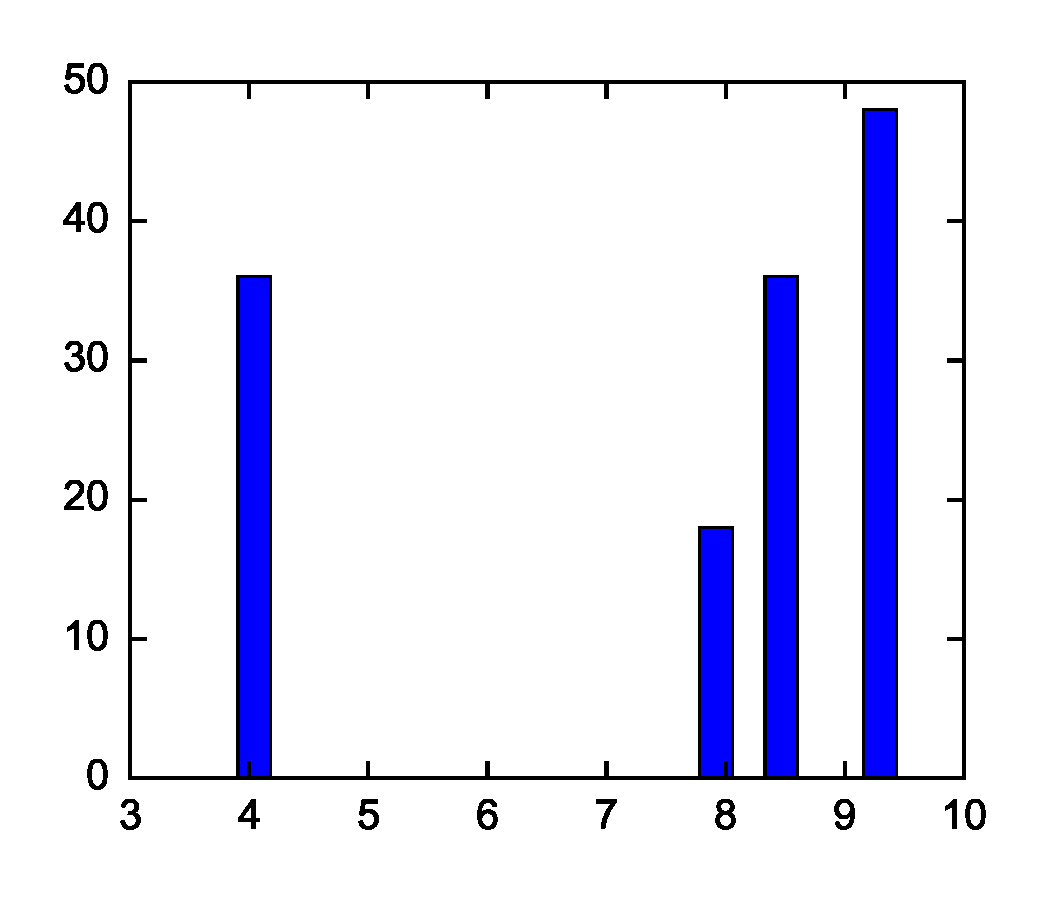
\includegraphics[width=0.5\textwidth]{Figures/neighbourHist.pdf}
%    \caption{A representative histogram of the neighbour separation distribution.}
%	\label{fig:neighbourHist}
%\end{figure}
%
%\begin{itemize}
%    \item{Figure \ref{fig:neighbourHist} shows an example distribution of the chromophore neighbour separation.}
%    \item{There is a strong peak at low separations, around 4-5\AA. These represent the closest neighbours to each chromophore in the system, which lie within the same stack.}
%    \item{Picking a clustering cut-off somewhere in between this peak and the next peak at $> 10$\AA (which represents next-nearest neighbours and/or neighbouring stacks) will ensure that only chromophores that lie within the same stack will be added to the cluster list.}
%    \item{The code dynamically determines the midpoint between the two peaks and uses this as the cut-off for each morphology. In all cases, the cut-off is $\sim 6$\AA.}
%    \item{Chromophores that lie within the cut-off are then deemed as being in the same stack, which includes periodic boundary conditions}
%\end{itemize}
%
%
%The stack locations are as follows, and the totals summarised in Table \ref{table:mob}.
%
%
%\begin{figure}[h!]\centering
%	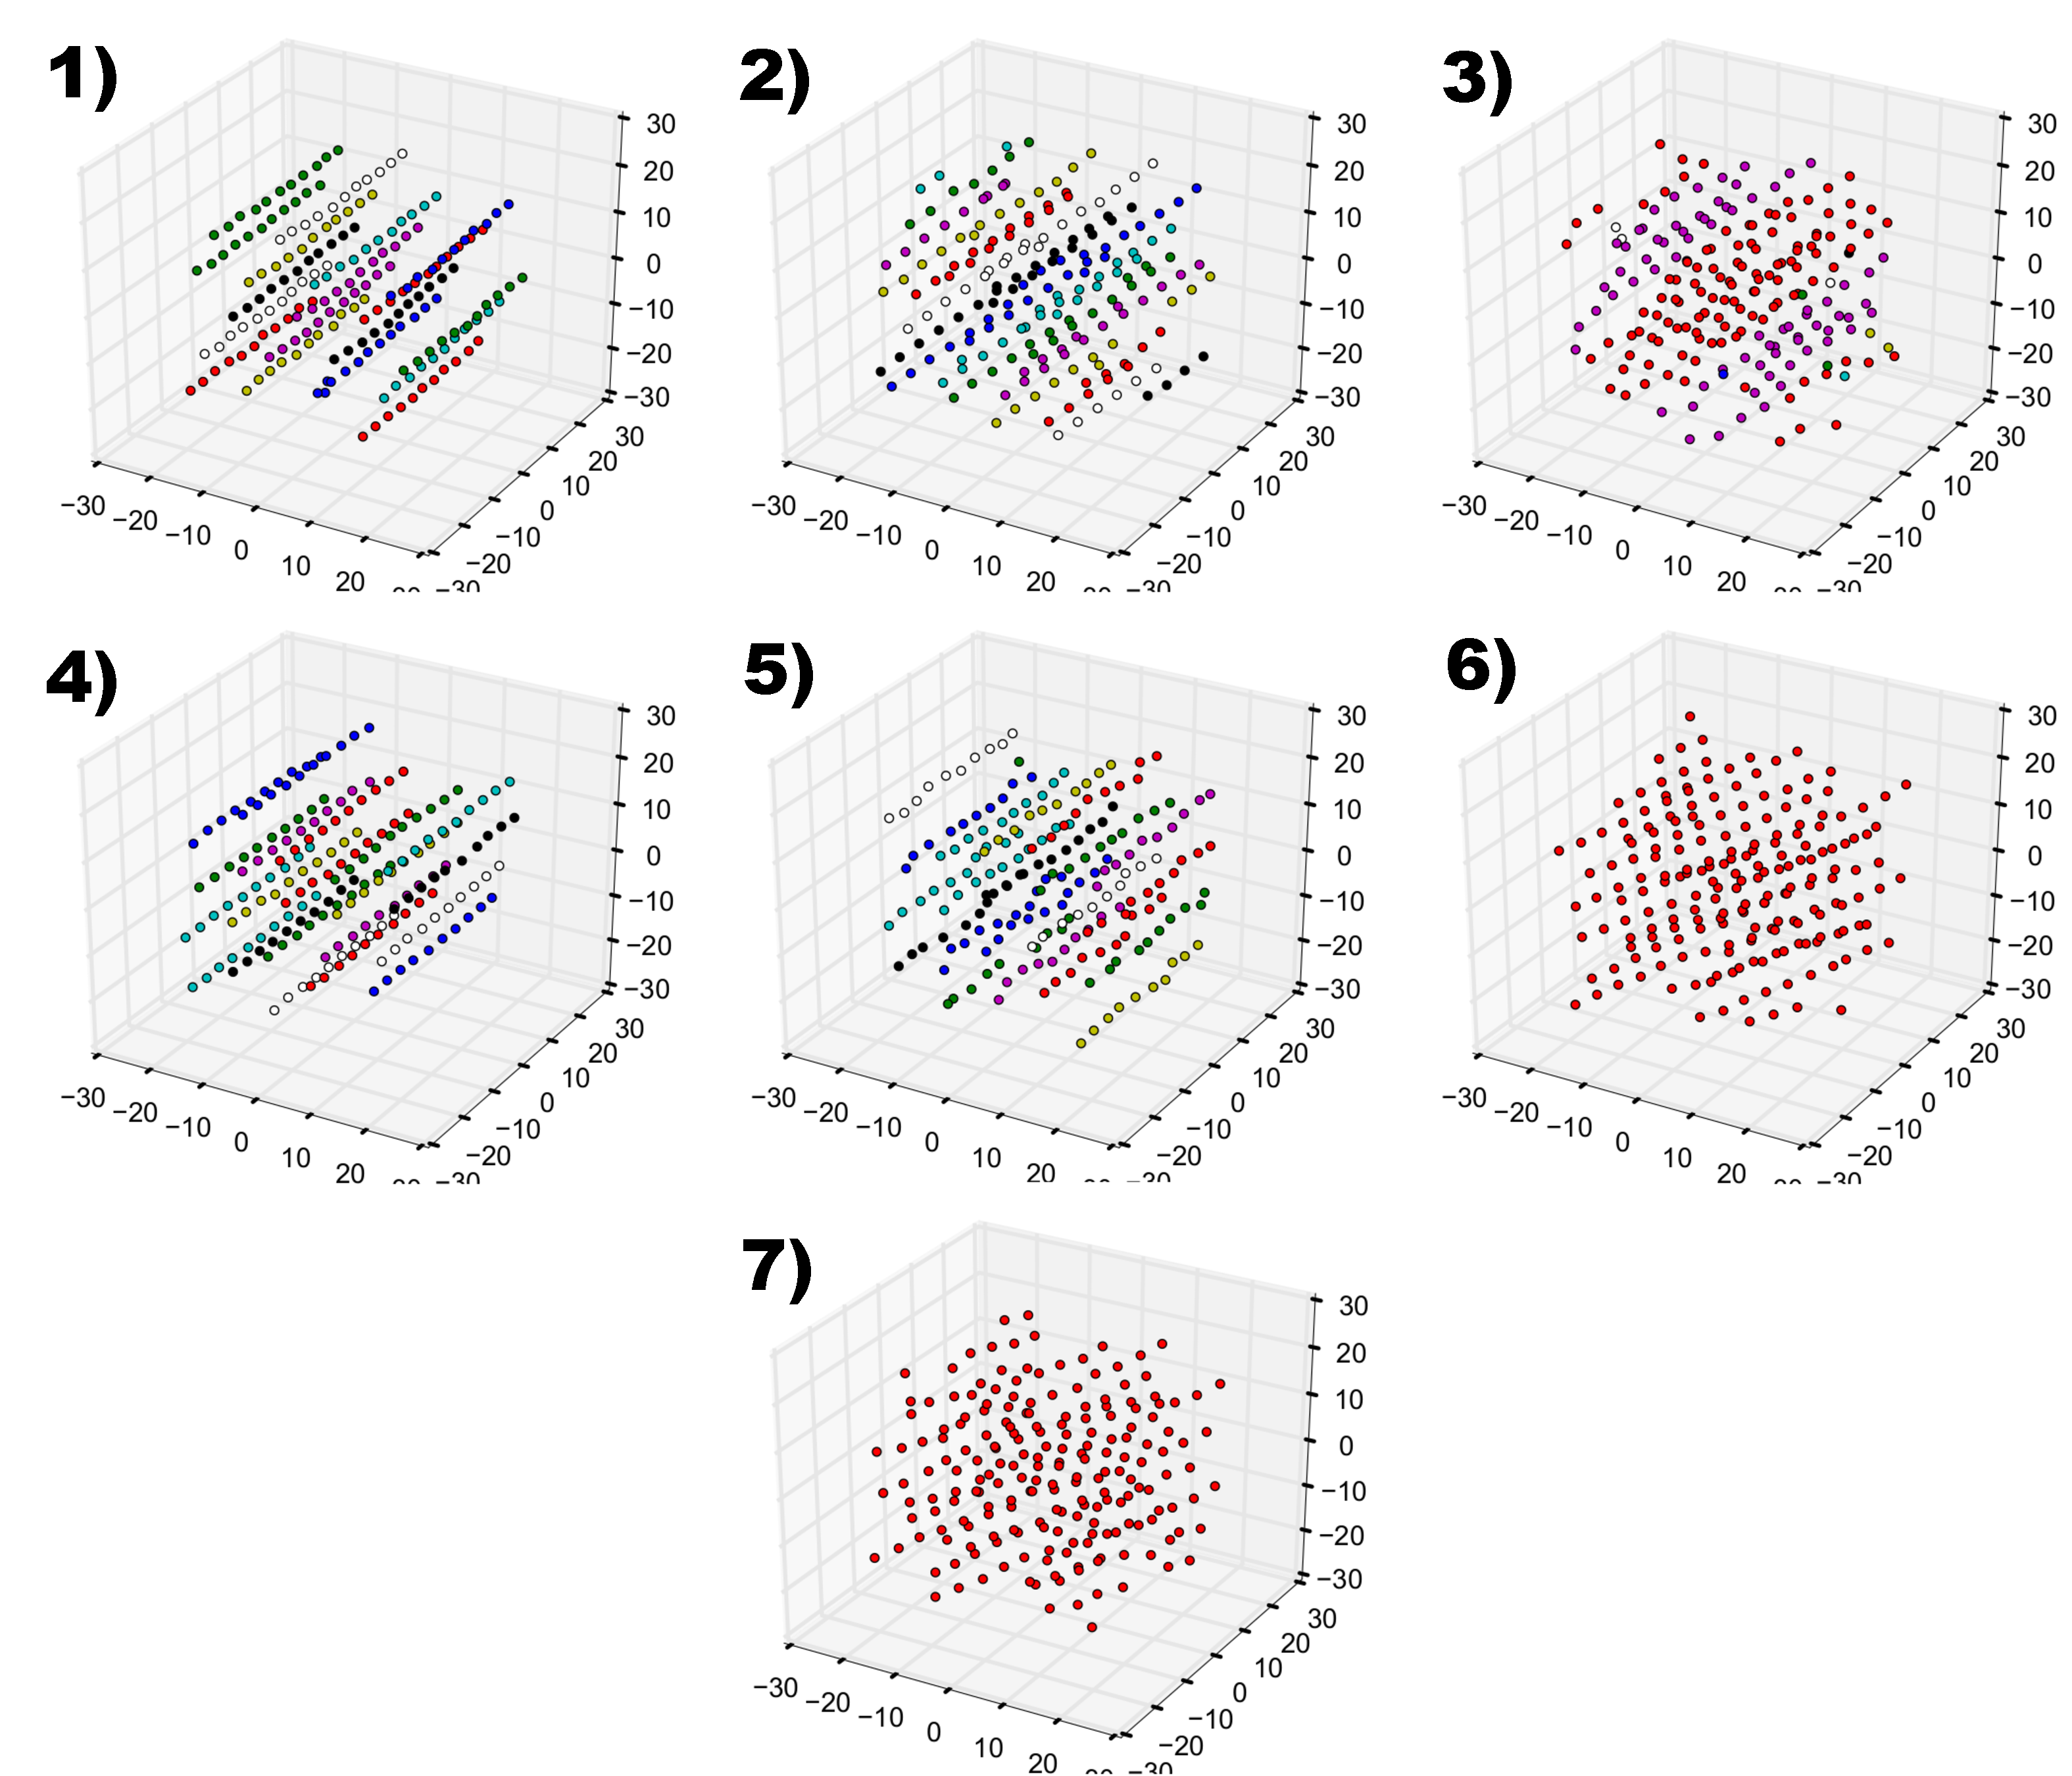
\includegraphics[width=\textwidth]{Figures/stacks.pdf}
%    \caption{The 3D visualisations of each stack in the PAH systems.}
%	\label{fig:stacks}
%\end{figure}
%
%
%\begin{itemize}
%    \item{The stack distributions look correct, and so it seems that the above method is sufficient to determine the quantity of stacks in the simulation.}
%    \item{Interestingly, it seems that while the PT does form a single-stack system, the `single-stack' PE systems that we look at actually contain 8 stacks (\textbf{2}) or 10 stacks (\textbf{3}).}
%    \item{In the case of \textbf{3}, one of the stacks is very large, and there are some `islands' due to spatial disorder in the system when compared to the eclipsed case. This could possibly be rectified by modifying the cutoff to include some of those islands, but it does suggest that \textcolor{red}{using the size of the largest stack in the system might be a good metric for quantifying the mobility trend}.}
%\end{itemize}
%
%\clearpage
%
%\subsection{Hopping Rate Distributions}
%
%Now that stacks are defined, we can now explore the difference in distribution between hops along the stack and between neighbouring stacks.
%\textcolor{red}{In particular, we're interested in why the Perylene results are odd.
%    PT appears to do everything that we'd expect:
%    \begin{enumerate}
%        \item{Eclipsed has higher mobility than Ordered}
%        \item{In the single-stack case, the anisotropy is significantly enhanced in eclipsed rather than disordered}
%        \item{The single-stack case has significantly higher mobility than the multi-stack case}
%    \end{enumerate}
%    However, in Perylene, trends 1) and 2) do not apply.
%}
%
%\begin{figure}[h!]\centering
%	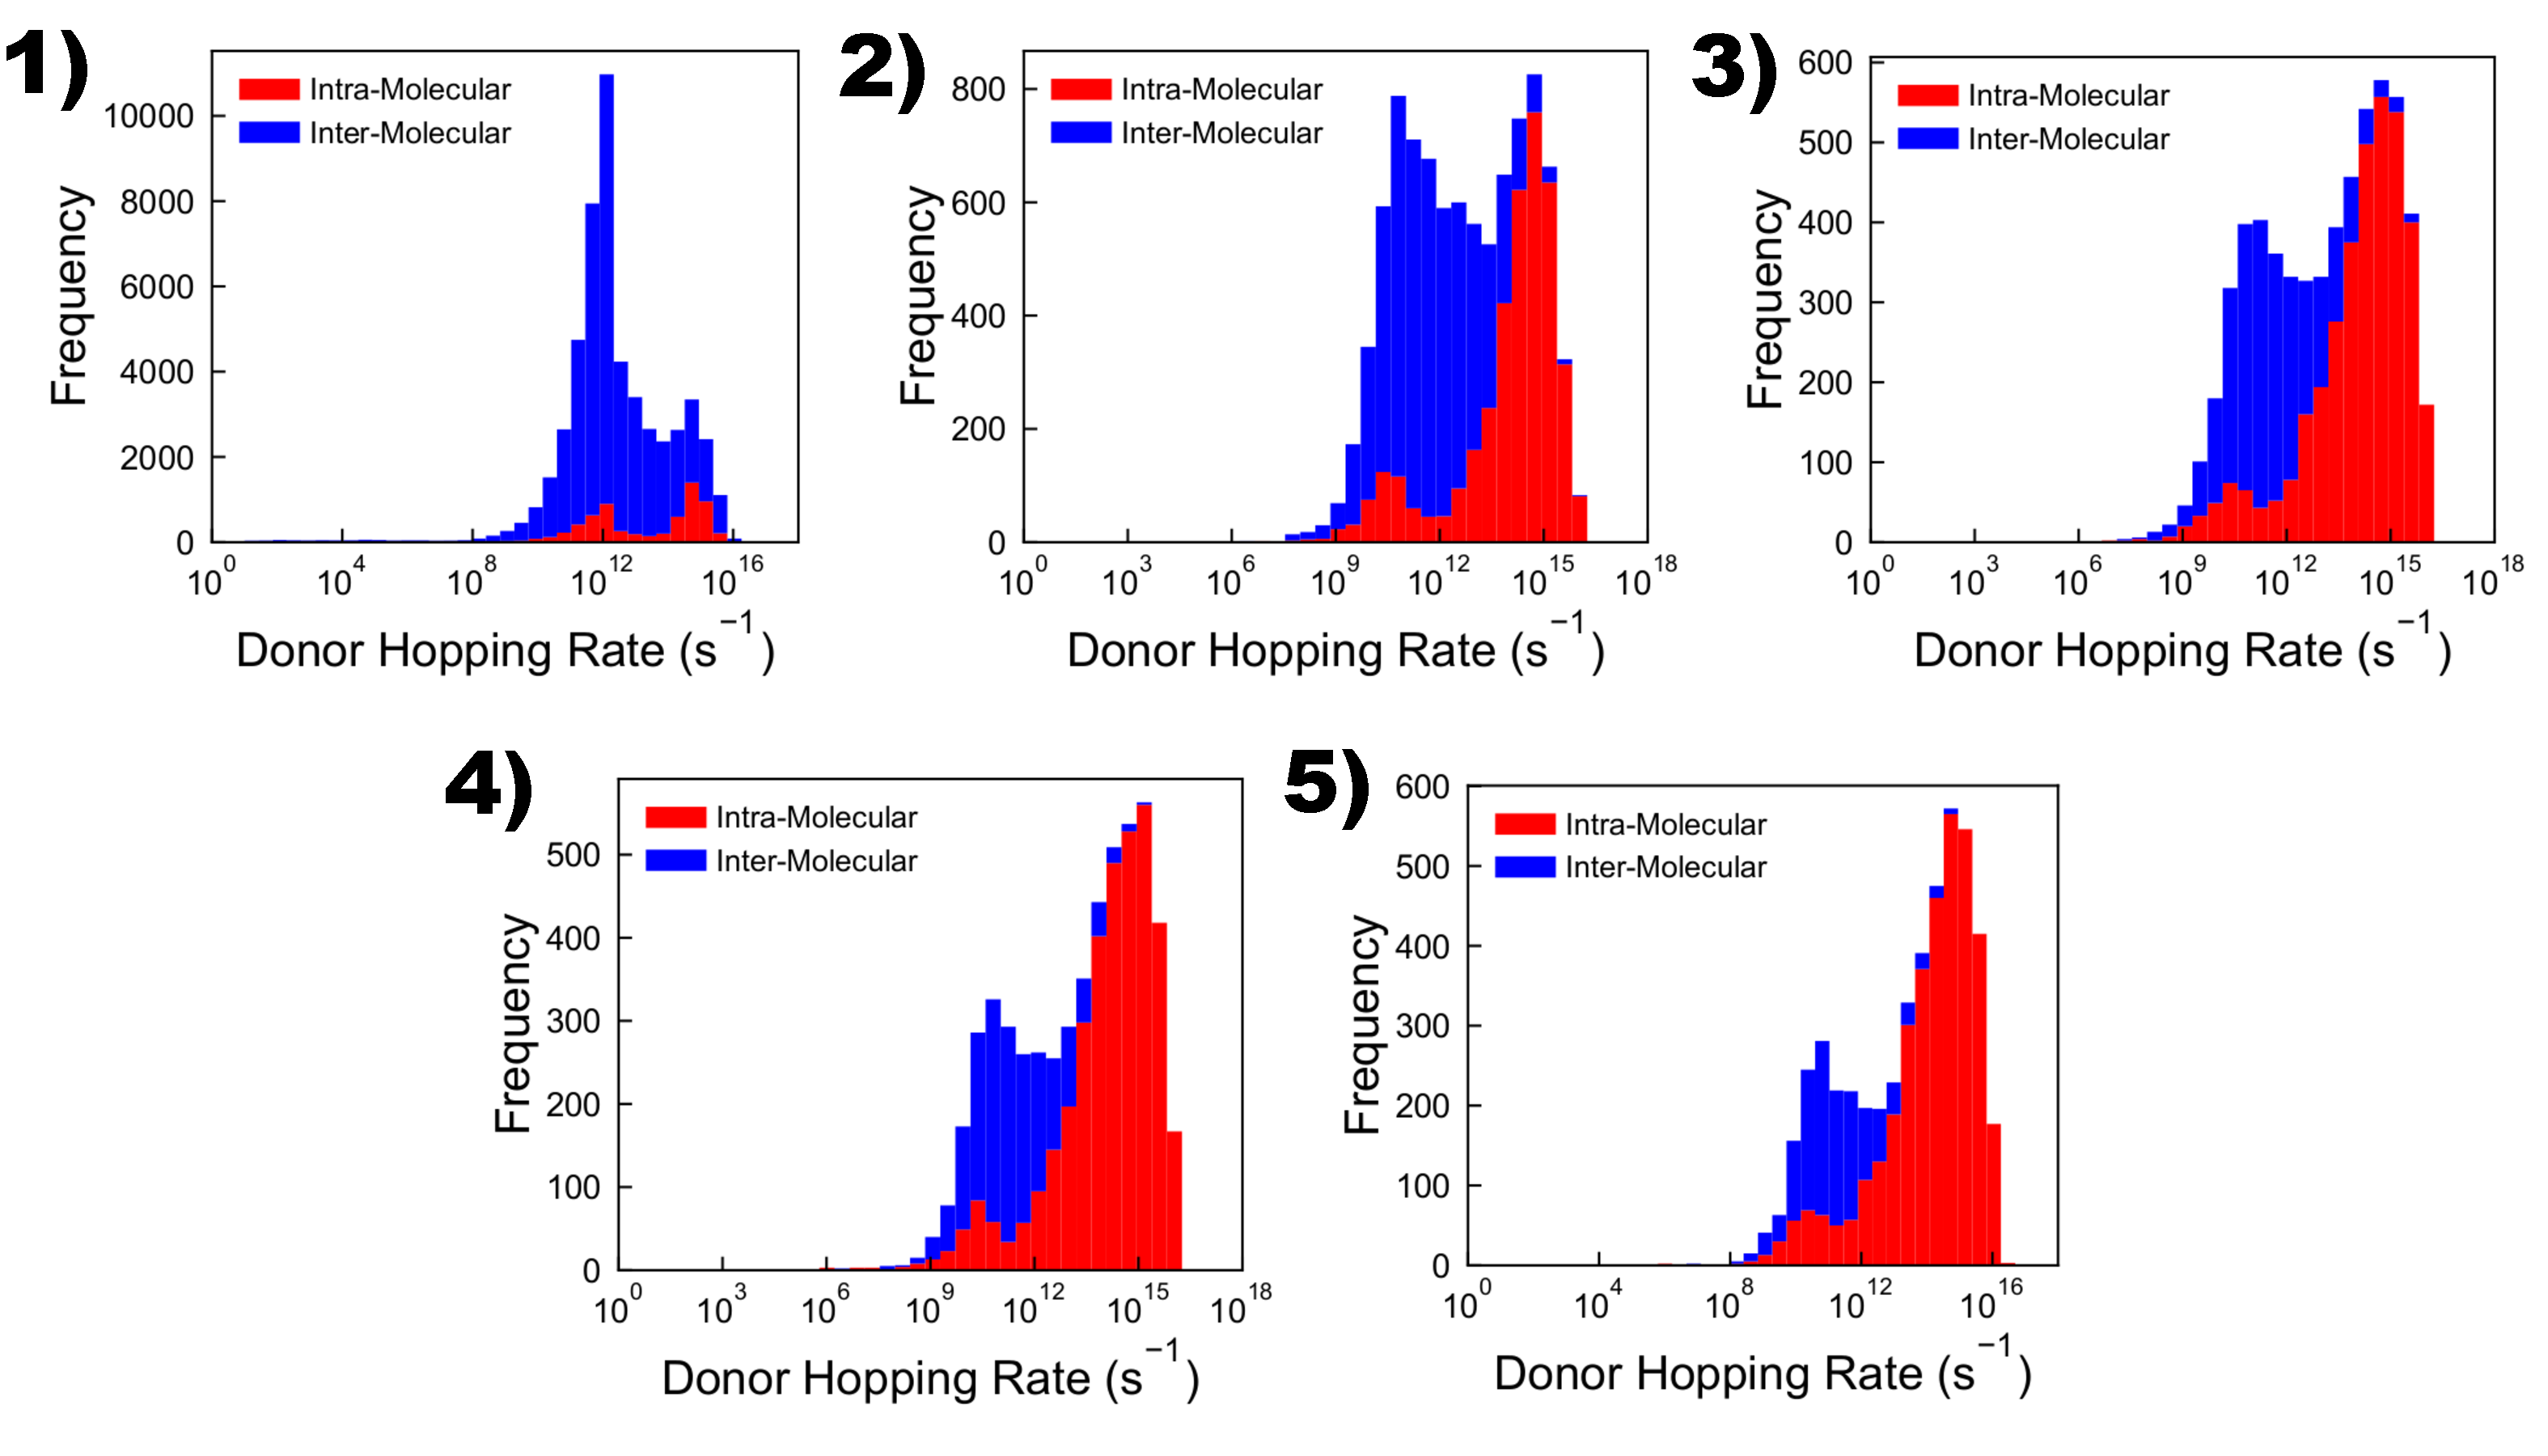
\includegraphics[width=\textwidth]{Figures/DonorHoppingRateMixed.pdf}
%    \caption{The hopping-rate distributions for hops executed by carriers within the morphologies \textbf{1} - \textbf{7}. Red bars showhops within the same stack, whereas the blue bars describe hops between stacks. The bars themselves are stacked on top of each other.}
%	\label{fig:HoppingRateMixed}
%\end{figure}
%
%\begin{itemize}
%    \item{The hopping rate distributions vary quite a lot! Some are single-mode, others bimodal, and one is tri-modal.}
%    \item{The modality of the peaks generally corresponds to nearest and next-nearest neighbour hops. The exceptions are:
%        \begin{itemize}
%            \item{\textbf{1}: which shows a third peak because the stacks are closely spaced, meaning that hopping to a nearby stack is more likely to occur than hopping to the next-nearest neighbour within the same stack.}
%            \item{\textbf{4}: the bimodal behaviour is somewhat visible in the intra-stack hops but is washed out by a large number of inter-stack hops that occur with unimodal rates.}
%            \item{\textbf{5}: As \textbf{4}, but with fewer inter-stack hops available (likely due to increased separation between the stacks due to structural disorder and paracrystallinity within the stack (this morphology is ordered instead of eclipsed)).}
%        \end{itemize}}
%    \item{In morphology \textbf{1}, the fastest hops (that KMC preferentially samples) occur along the stack, with very few hops in between stacks.
%        This explains the high anisotropy of this system, and also why its mobility is so high (intra-stack hops occur more quickly).}
%    \item{Morphology \textbf{2} also has a high ratio of intra-to-inter-stack hopping at the fastest rates, however its anisotropy is significantly reduced.
%        This is likely because there is more of a mix of intra- and inter-stack hops at slightly lower rates, but still within the sampling window (rates $> 10^{13}$).}
%
%\end{itemize}


\bibliography{refs}
\bibliographystyle{unsrt}


\end{document}
